\chapter{Разработка информационной технологии прогнозирования временных рядов, прототипа ее программной реализации на основе нечеткой модели и оценка работоспособности}\label{ch:ch4}

\section{Библиотека с параллельной реализацией нечеткого вывода на основе технологии CUDA}

Реализация информационной технологии прогнозирования для предложенного метода на основе нечеткой модели, согласно разработанным алгоритмам, является композицией последовательности этапов вычислений различной сложности. Этап, содержащий наибольший объем вычислений, включает в себя процедуру нечеткого вывода. Его реализация потребует организации эффективного использования ресурсов аппаратной платформы для организации вычислений по разработанным алгоритмам.

Согласно схемам \cref{fig:nfs-ftv-and-defuz-meom-with-defuz-demo}, изображенным во \ref{ch:ch2}-м разделе, для достижения высокой производительности процедура нечеткого вывода может быть скомпонована из последовательности параллельных участков независимых вычислений и сверток. Распространенным подходом реализации параллельных вычислений является использование вычислений на графическом процессоре.

Для удобства реализация выполнялась не посредством прямого использованием API библиотеки CUDA, а с помощью библиотеки реализации высокопроизводительных вычислений - \textbf{Kokkos} \cite{KokkosWiki, KokkosCarterEdwards20143202}, предназначенной для портативного и эффективного параллельного программирования на различных аппаратных архитектурах, включая многоядерные процессоры, графические процессоры NVIDIA/AMD и другие ускорители. Интерфейс библиотеки позволяет абстрагироваться от деталей низкоуровневого параллелизма, позволяя разработчикам писать код на C++ с одним исходным кодом, который может быть оптимизирован для различных платформ без существенных изменений. 
Ключевые функциональные возможности библиотеки упростившие выполнение программной реализации разработанного выше метода:
\begin{itemize}
	\item Модели параллельного выполнения: абстрагирование параллельных циклов (например, \lstinline|parallel_for|, \lstinline|parallel_reduce|) и рабочих процессов на основе задач.  
	\item Управление памятью: автоматизированная обработка пространств памяти (например, между хостом и устройством) и расположением данных для оптимизации схем доступа и минимизации объема передаваемых данных.  
	\item Поддержка серверной части: интеграция с такими моделями программирования, как CUDA, HIP, OpenMP и SYCL, для обеспечения кроссплатформенной совместимости.
	\item Переносимость производительности: Обеспечивает эффективное использование ресурсов (потоки, векторизация) с учетом особенностей каждой архитектуры.
\end{itemize}

Kokkos широко используется в научных вычислениях и HPC-приложениях, упрощая разработку масштабируемых кодов при сохранении производительности на постоянно развивающемся оборудовании. 

\begin{figure}[ht]
	\centering
	\includegraphics[scale=0.95]{fuzzy-infer-flowchart}
	\caption{Блок схема процедуры нечеткого логического вывода на основе нечеткого значения истинности.}
	\label{fig:fuzzy-infer-flowchart}
\end{figure}

При выполнении процедуры нечеткого вывода для набора входных данных можно выполнять процедуру вывода по каждому входному экземпляру независимо, то есть параллельно. Сам алгоритм нечеткого вывода не предусматривает наличия промежуточной информации, которой бы нужно было обмениваться между вычислениями по другим экземплярам входных данных. Тогда, поскольку алгоритм нечеткого вывода для каждого экземпляра входных данных можно реализовать при ограниченном небольшом объеме входных и промежуточных данных, имеет смысл разместить эти данные в памяти предоставляющей наибольшую скорость доступа к данным, которая в технологии CUDA соответствует разделяемой памяти внутри CUDA-блока, а сами вычисления над этими данными также реализовать внутри этого CUDA-блока.

Время нечеткого вывода может быть сокращено за счет уменьшения времени работы отдельного CUDA-блока путем увеличения количества параллельных CUDA-нитей. Тогда планировщик  \textit{потокового мультипроцессора} (\textit{streaming multiprocessor}) сможет распределять инструкции между доступными арифметико-логическими модулями, обеспечивая \textit{instruction pipelining}, или сократить амортизированное время задержки (\textit{latency}) при выполнении длительной инструкции подгрузки данных из глобальной памяти графического процессора. Однако с другой стороны слишком большое количество нитей внутри CUDA-блока упрется в ограниченное количество ригистровой памяти и ограниченное количество арифметико-логических модулей внутри потокового мультипроцессора (распределяемых между нитями 4-мя планировщиками на большинстве версий \textit{наборов вычислительных возможностей (compute capabilities)}. Ограниченность объема разделяемой памяти на один потоковый мультипроцессор также может ограничить предельное число CUDA-блоков, размещаемых в одном потоком мультипроцессоре, Согласно документации CUDA, устройства с набором вычислительных возможностей версии 7.5 (и некоторых более низких версий) максимальный объем разделяемой памяти на одном потоковом мультипроцессоре равен 64 кБ, а на устройствах с набором вычислительных возможностей более высокой версии --- предусмативается 100 - 164 кБ разделяемой памяти. Рациональное использование только необходимого объема разделяемой памяти позволит планировщику на графическом процессоре поставить на исполнение сразу несколько CUDA-блоков на один потоковый мультипроцессор.

\begin{figure}[ht]
	\centering
	\includegraphics[scale=0.7]{cuda-shared-memory-map}
	\caption{Карта разделяемой памяти одного CUDA-блока нечеткого логического вывода на основе нечеткого значения истинности при использовании дефаззификации MeOM.}
	\label{fig:ftv-infer-cuda-shared-memory-map}
\end{figure}

Суммарный объем разделяемой памяти, необходимый для работы процедуры нечеткого вывода для одного входного экземпляра, складывается из объемов памяти используемых в этом выводе данных. Основной вклад в этот объем делают компоненты данных:
\begin{itemize}
	\item параметры ф. п. $N$ правил при $n$ входах (2 параметра для гауссовой ф-и): $(\text{\lstinline|sizeof float|}) \times (n+1) \times N \times 2$;
	\item параметры ф. п. входного экземпляра данных при $n$ входах (2 параметра для гауссовой ф-и): $(\text{\lstinline|sizeof float|}) \times (n+1) \times 2$;
	\item значения свертки НЗИ для $N$ правил при размере расчетной сетки равному $D_{ftv}$: $(\text{\lstinline|sizeof float|}) \times D_{ftv} \times N$ и промежуточные данные:
	\begin{itemize}
		\item индексы координат расчетной сетки с максимальным значением НЗИ каждому из $N$ правил и $n$ входов: $(\text{\lstinline|sizeof char|}) \times n \times N \times 2$;
		\item максимальные значения НЗИ на текущей итерации свертки НЗИ по каждому из $N$ правил и $n$ входов: $(\text{\lstinline|sizeof float|}) \times n \times N \times 2$;
	\end{itemize}
	\item популяции из $P$ координат $y^{(p)}$, скоростей изменения координат $v^{(p)}$, значений выходной ф. п. $\mu_{B'}(y^{(p)})$, координат локальных оптимумов $y^{*(p)}$, значений выходной ф. п. в локальных оптимумах $\mu_{B'}(y^{*(p)})$ (5 популяций): $(\text{\lstinline|sizeof float|}) \times P \times 5$.
\end{itemize}
Последний пункт приведен для случая использования \textit{MeOM} в качестве метода дефаззификации.

При нечетком выводе для одного входного экземпляра в одном CUDA-блоке, значимая доля вычислительного времени будет потрачена на загрузку базы правил из глобальной памяти в разделяемую память, а, в случае когда данные одного CUDA-блока будет занимать значимую долю доступной разделяемой памяти, число <<подменных>> CUDA-блоков на один потоковый процессор будет низким. Лучшим решением будет реализация <<долгоживущих>> CUDA-блоков, каждый из которых занимает большую часть разделяемой памяти. В таком случае база правил подгружается в разделяемую память один раз, а нечеткий вывод производится сразу для пакета экземпляров входных данных. Карта организации разделяемой памяти внутри одного такого CUDA-блока изображена на рисунке \cref{fig:ftv-infer-cuda-shared-memory-map}.

При достаточном размере пакета данных, обрабатываемых внутри одного CUDA-блока, нечеткий вывод по отдельному экземпляру выгодно реализовать внутри отдельного набора из 32-х нитей (\textit{warp}), которые исполняются единым пакетом нитей вычисления. Такой способ организации вычислений позволит практически полностью избавиться от барьерной синхронизации между нитями всего CUDA-блока с использованием \lstinline|__syncthreads()|, а для реализации эффективной свертки внутри набора из 32-х нитей CUDA предоставляет набор \textit{intrinsic}-функций --- \lstinline|__shfl()|, \lstinline|__shfl_down()|, \lstinline|__shfl_up()| и \lstinline|__shfl_xor()|.

Из описанного ранее функционала библиотеки Kokkos для размещения и доступа к данным в разделяемой памяти CUDA-блока крайне удобно использовать \lstinline|Kokkos::View| с опорой на широко эксплуатируемую в среде C++ разработчиков идиому RAII (Resource acquisition is initialization --- получение некоторого ресурса неразрывно совмещается с инициализацией, а освобождение --- с уничтожением объекта), которая позволяет избавиться от необходимости <<ручного>> вычисления адресов и смещений, располагаемых в разделяемой памяти, программных объектов, что особенно актуально при переиспользовании сегментов разделяемой памяти, занимаемых временными данными, в дальнейших шагах алгоритма.

Для выделения памяти c помощью \lstinline|Kokkos::View| требуется получить дескриптор разделяемой памяти текущего CUDA-блока с помощью вызова \lstinline|Kokkos::TeamHandleConcept<>::team_shmem()| , который описывает текущее состояние разделяемой памяти данного CUDA-блока.

Поскольку вычисление свертки НЗИ для всех правил нечеткой системы составляет половину сложности алгоритма нечеткого вывода и в последствии будет неоднократно использооваться при агрегации правил, необходимо обеспечить единоразовое вычисление функции принадлежности свертки НЗИ (или ее аппроксимации), в результате которого будут известны значения последней на всей ее области определения.

\subsection{Вычисление нечеткого значения истинности посредством дискретизации}\label{sec:ch3/sect1}

При реализации вычисления НЗИ, когда функции принадлежности нечетких множеств $A$ и $A'$ заданы гауссовыми функциями, может возникнуть сложность, когда ф. п. НЗИ вырождается в близкий к некоторой асимптоте (горизонтальной или вертикальной) вид. Для изучения условий возникновения таких ситуаций перепишем формулу (\ref{eqn:ftv-gauss-expanded}) ниже и обозначим ее составные компоненты через $\alpha$, $\beta$, $\phi(v)$:
\begin{equation*}
	\exp\left(-\left(\underbrace{\frac{a_1-a_2}{b_2}}_{\alpha}\pm\underbrace{\frac{b_1}{b_2}}_{\beta}\underbrace{\sqrt{-\ln v}}_{\phi(v)}\right)^2\right).
	\label{eqn:ftv-gauss-components-markup}
\end{equation*}
Тогда вычисление значения (\ref{eqn:ftv-gauss-expanded}) можно представить в виде композиции функций
\begin{equation}
	\mu_{CP(A,A')}(v)=\exp(-z(v)^2),
	\label{eqn:ftv-gauss-exp-z}
\end{equation}
и
\begin{equation}
	z(v)=\alpha \pm \beta \phi(v).
	\label{eqn:ftv-gauss-phi}
\end{equation}

\pgfplotsset{
	membership axes/.style={
		%width=0.45\textwidth,
		%height=0.45\textwidth,
		scale only axis,
		domain=0:1,
		samples=100,
		every axis plot/.append style={smooth},
		axis lines=middle,
		xmin=0, xmax=1,
		ymin=0, ymax=1,
		xticklabel style={font=\tiny, inner sep=1pt, outer sep=0pt},
		yticklabel style={font=\tiny, inner sep=1pt, outer sep=0pt},
		legend style={font=\small},
	}
}


\begin{figure}[ht]
	\centering
	\begin{minipage}[t]{0.48\textwidth}
		\centering
		\begin{tikzpicture}
			\begin{axis}[
				membership axes,
				domain=0:5,
				samples=100,
				xmax=5,
				]
				\addplot [blue, thick] {exp(-(x^2))};
			\end{axis}
		\end{tikzpicture}
		\caption{График функции $\exp(-z^2)$}
		\label{fig:ftv-exp-component}
	\end{minipage}
	\hfill
	\begin{minipage}[t]{0.48\textwidth}
		\centering
		\begin{tikzpicture}
			\begin{axis}[
				membership axes,
				samples=100,
				ymax=3,
				]
				\addplot [blue, thick] {sqrt(-ln(x))};
			\end{axis}
		\end{tikzpicture}
		\caption{График функции $\phi(v)=\sqrt{-\ln v}$}
		\label{fig:ftv-phi-component}
	\end{minipage}
\end{figure}

Для иллюстрации условий возникновения описанных вырождений функции (\ref{eqn:ftv-gauss-expanded}) графики функций (\ref{eqn:ftv-gauss-exp-z}) и (\ref{eqn:ftv-gauss-phi}) при $\alpha = \beta = 1$ приведены на рисунках \cref{fig:ftv-exp-component} и \cref{fig:ftv-phi-component} соответственно. Из рисунка \cref{fig:ftv-phi-component} видно, что вырождение выражения (\ref{eqn:ftv-gauss-exp-z}) в близкий к асимптоте вид возможно при очень больших или очень малых значениях $\alpha$ и $\beta$. Данное наблюдение проиллюстрировано на рисунке \cref{fig:ftv-gauss-corner-cases}.

\begin{figure}[htbp]
	\centering
	
	% First row
	\begin{subfigure}[t]{0.48\textwidth}
		\newcommand{\aOne}{1}
		\newcommand{\bOne}{0.2}
		\newcommand{\aTwo}{0.95}
		\newcommand{\bTwo}{1}
		\centering
		\begin{tikzpicture}
			\begin{axis}[
				membership axes,
				samples=1000,
				]
				\addplot [blue, thick] {gauss(\aOne-2*\bOne*sqrt(-ln(x)), \aTwo, \bTwo)};
				\draw [blue, thick] (0.001464278918,0.8) -- (0.0001,0);
			\end{axis}
		\end{tikzpicture}
		\caption{$\mu_{CP(A, A')}(v)$ при $\alpha \approx 0, \beta \approx 0$}
		\label{fig:ftv-corner-cases-zeroBeta-1}
	\end{subfigure}
	\hfill
	\begin{subfigure}[t]{0.48\textwidth}
		\newcommand{\aOne}{1}
		\newcommand{\bOne}{1}
		\newcommand{\aTwo}{0.95}
		\newcommand{\bTwo}{0.1}
		\centering
		\begin{tikzpicture}
			\begin{axis}[
				membership axes,
				samples=1000,
				]
				\addplot [blue, thick] {gauss(\aOne-2*\bOne*sqrt(-ln(x)), \aTwo, \bTwo)};
			\end{axis}
		\end{tikzpicture}
		\caption{$\mu_{CP(A, A')}(v)$ при $\alpha \approx 0, \beta \gg 0$}
		\label{fig:ftv-corner-cases-largeBeta-1}
	\end{subfigure}
	
	% Second row
	\begin{subfigure}[t]{0.48\textwidth}
		\newcommand{\aOne}{3.34}
		\newcommand{\bOne}{0.02}
		\newcommand{\aTwo}{5}
		\newcommand{\bTwo}{1}
		\centering
		\begin{tikzpicture}
			\begin{axis}[
				membership axes,
				samples=1000,
				domain=0.001:1,
				]
				\addplot [blue, thick] {gauss(\aOne+2*\bOne*sqrt(-ln(x)), \aTwo, \bTwo)};
			\end{axis}
		\end{tikzpicture}
		\caption{$\mu_{CP(A, A')}(v)$ при $|\alpha| \gg 0, \beta \approx 0$}
		\label{fig:ftv-corner-cases-zeroBeta-2}
	\end{subfigure}
	\hfill
	\begin{subfigure}[t]{0.48\textwidth}
		\newcommand{\aOne}{3.34}
		\newcommand{\bOne}{1}
		\newcommand{\aTwo}{5}
		\newcommand{\bTwo}{0.02}
		\centering
		\begin{tikzpicture}
			\begin{axis}[
				membership axes,
				samples=1000,
				domain=0.001:1,
				]
				\addplot [blue, thick] {gauss(\aOne+2*\bOne*sqrt(-ln(x)), \aTwo, \bTwo)};
			\end{axis}
		\end{tikzpicture}
		\caption{$\mu_{CP(A, A')}(v)$ при $|\alpha| \gg 0, \beta \gg 0$}
		\label{fig:ftv-corner-cases-largeBeta-2}
	\end{subfigure}
	
	% Third row
	\begin{subfigure}[t]{0.48\textwidth}
		\newcommand{\aOne}{1}
		\newcommand{\bOne}{0.1}
		\newcommand{\aTwo}{0.3}
		\newcommand{\bTwo}{0.1}
		\centering
		\begin{tikzpicture}
			\begin{axis}[
				membership axes,
				samples=1000,
				]
				\addplot [blue, thick] {gauss(\aOne-2*\bOne*sqrt(-ln(x)), \aTwo, \bTwo)};
				\draw [blue, thick] (0.0014,0.4) -- (0.0001,1);
			\end{axis}
		\end{tikzpicture}
		\caption{$\mu_{CP(A, A')}(v)$ при $|\alpha| \gg 0, \beta = 1$}
		\label{fig:ftv-corner-cases-oneBeta}
	\end{subfigure}
	
	\caption{Случаи вырождения ф. п. НЗИ в близкий к асимптоте вид.}
	\label{fig:ftv-gauss-corner-cases}
\end{figure}

В ситуациях, изображенных на рисунках \cref{fig:ftv-corner-cases-zeroBeta-1, fig:ftv-corner-cases-largeBeta-1, fig:ftv-corner-cases-largeBeta-2, fig:ftv-corner-cases-oneBeta}, функция принадлежности НЗИ имеет своей асимптотой вертикальную прямую $v = v_0$. При реализации вычисления НЗИ с использованием расчетной сетки, связанная с тем, что ф. п. НЗИ в точке может быть вообще не определена (рис. \cref{fig:ftv-corner-cases-zeroBeta-1, fig:ftv-corner-cases-oneBeta}) или ф. п. НЗИ в точке $v_0$ имеет значение сильно отличающееся от значений в ближайших точках расчетной сетки $v_1$ и $v_2$ при $v_0 \in (v_1, v_2)$, из-за чего значение НЗИ в бесконечно малой окрестности точки $v_0$ будет упущено.

Из рисунка \cref{fig:ftv-exp-component} видно, что максимальное значение выражения (\ref{eqn:ftv-gauss-exp-z}), равное 1, достигается при $z = 0$, а из рисунка \cref{fig:ftv-phi-component} видно, что функция (\ref{eqn:ftv-gauss-phi}) обязательно пересекает ось абсцисс, то есть максимальное значение ф. п. НЗИ всегда равно 1. Тогда для решения проблемы <<просеивания>> значения $\mu_{CP(A, A')}(v_0)$ сквозь точки расчетной сетки можно вычислить координату точки $v_0$, в которой функция (\ref{eqn:ftv-gauss-expanded}) принимает свое максимальное значение, а затем положить значение в ближайшей к $v_0$ точке расчетной сетки равным этому максимуму, то есть значению 1. Для этого выразим аналитически значение $v_0$, в котором (\ref{eqn:ftv-gauss-expanded}) принимает значение 1.

\begin{align}
	\exp\left(-\left(\frac{(a_1-a_2)\pm b_1\sqrt{-\ln v_0}}{b_2}\right)^2\right) &= 1 \nonumber \\
	\exp\left(-\left(\frac{(a_1-a_2)\pm b_1\sqrt{-\ln v_0}}{b_2}\right)^2\right) &= \exp(0) \nonumber \\
	\frac{(a_1-a_2)\pm b_1\sqrt{-\ln v_0}}{b_2} &= 0 \nonumber \\
	\pm b_1\sqrt{-\ln v_0} &= a_1-a_2 \nonumber \\
	\sqrt{-\ln v_0} &= \pm\frac{a_1-a_2}{b_1} \nonumber \\
	\ln v_0 &= -\left(\frac{a_1-a_2}{b_1}\right)^2 \nonumber \\
	v_0 &= \exp\left(-\left(\frac{a_1-a_2}{b_1}\right)^2\right) \label{eqn:ftv-gauss-argmax}
\end{align}

Внедрение выражения (\ref{eqn:ftv-gauss-argmax}) в алгоритм вычисления НЗИ позволит обеспечить соответствие определению дискретизированного представления ф. п. НЗИ. \todo{Строго говоря ф. п. на рисунке определена в точке $v_0$ и не требует\dots.} НЗИ с функцией принадлежности, имеющей горизонтальную асимптоту, как на рисунке \cref{fig:ftv-corner-cases-zeroBeta-2} может вызвать сложность при построении алгоритма вычисления НЗИ на использовании метода градиентного спуска вместо дискретизации с фиксированным шагом расчетной сетки.

Вычисление нечеткого значения истинности для каждого правила по каждому входу отдельно предварительным этапом приведет к линейному увеличению объема необходимой памяти. Поскольку вычисление НЗИ является довольно легкой операцией, лучшим решением будет встраивание вычисления НЗИ по каждому входу в процедуру свертки НЗИ.

Формула (\ref{}) предлагает построение процедуры свертки НЗИ в виде дерева попарных сверток, для сохранения промежуточных результатов которых потребуется выделение объема памяти, также имеющего фактически линейный порядок зависимости от количества входов нечеткой системы. Возвращаясь к формуле (\ref{}) свертки НЗИ по входам в [] предложен параллельный алгоритм свертки НЗИ на расчетной сетке с постоянным шагом. Данный алгоритм итеративно вычисляет значение свертки НЗИ в каждой точки расчетной сетки продвигаясь от точки в пространстве истинности 1 к точке 0. Для каждого правила отдельно потребуется объем памяти, необходимый для сохранения значений свертки НЗИ в каждой точке расчетной сетки и для сохранения текущего максимального значения НЗИ по каждому входу на данной итерации алгоритма.

Преимуществом такого подхода представления НЗИ в программе является возможность быстрого нахождения значения функции принадлжености НЗИ в некоторой точке пространства истинности. Пара ближайших к этой точке позиций в массиве значений НЗИ на расчетной сетке определяется на основе значения фиксированного шага расчетной сетки. Для вычисления непосредственно ззначения НЗИ используется линейная интерполяция для найденной пары.

Поскольку при небольшом количестве входных переменных нечеткой системы большие участки расчетной сетки ф. п. свертки НЗИ соответствуют ф. п. НЗИ по одному из входов, при том же объеме памяти, необходимой для хранения результа сверки НЗИ, можно перейти к переменному шагу расчетной сетки с увеличением сложности функции аппроксимации участков ф. п. свертки НЗИ, принадлежащий ф. п. НЗИ одного из входов. Схема вычислений такого алгоритма схожа со схемой алгоритма при использовании постоянного шага расчетной сетки, а на каждой итерации определяется точка \dots

Ввиду необходимости использования большой размерности расчетной сетки для получения высокой точности дискретизации для размещения результата свертки НЗИ потребуется существенный объем разделяемой памяти. Например, при использовании для задания вычисленных значений вещественных чисел одинарной точности (4 байта) и размерности расчетной сетки равной 100 сохранение результата свертки НЗИ в нечеткой системе с 50 правилами в базе правил потребуется $4\textrm{ байта}\times 100 \times 50 = 20000\textrm{ байт}$ разделяемой памяти.

%\begin{figure}[hbt]
%	\centering
%	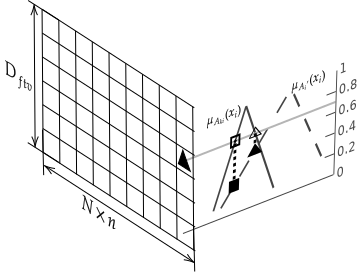
\includegraphics[width=0.6\textwidth]{ftv-opengl-computation.pdf}
%	\label{ftv-opengl-computation}
%\end{figure}
%
%\begin{figure}[hbt]
%	\centering
%	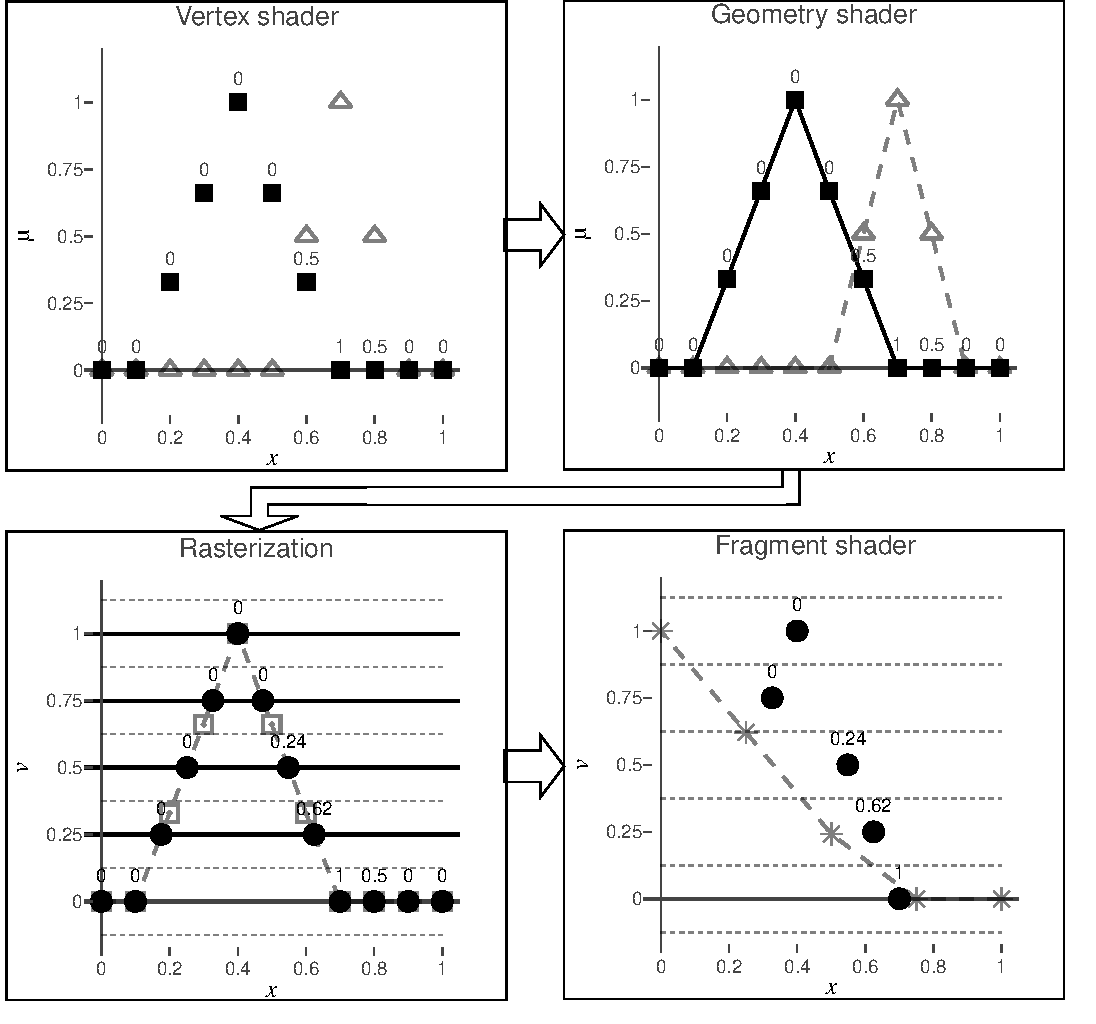
\includegraphics[width=1.0\textwidth]{ftv-opengl-computation-pipeline.pdf}
%	\label{ftv-opengl-computation-pipeline}
%\end{figure}



\subsection{Реализация обертки в Python-модуль}

Для ускорения процесса отладки и тестирования, выполненная на языке C++ (CUDA) реализация нечеткой модели собирается компилятором NVCC в динамически подключаемую библиотеку (\textit{*.so} (\textit{shared object}) файл в Linux). Реализованная на языке C часть Python-обертки библиотеки выполняет поиск файла библиотеки и символов в нем уже при запуске использующей эту библиотеку программы.

На сегодняшний день язык программирования Python занял позицию отраслевого стандарта в научных исследованиях и задачах анализа данных  Это обеспечено прежде всего удобным синтаксисом и легкостью интеграции большим многообразием высокопроизводительных библиотек научных вычислений, реализованных на языках с прямым управлением аппаратными ресурсами. Среди инструментов обеспечивающих реализацию механизма FFI в языке Python простым в использовании является инструмент Cython. Этот компилируемый метаязык расширяет парадигму Python, вводя статическую типизацию и структуры данных, характерные для системного программирования, что обеспечивает прозрачное описание C++ API. Современные инструменты пакетирования, включая обновленные версии setuptools, реализуют стандартизированные механизмы (PEP-517) для автоматизации включения Cython-компонентов в Python-пакеты.

\begin{figure}[ht]
	\centering
	\includegraphics[width=\linewidth]{application-schema-diagram}
	\caption{Схема использования библиотеки для нечеткого моделирования и прогнозирования временных рядов.}
	\label{fig:application-schema-diagram}
\end{figure}


\section{Оценка работоспособности разработанного метода прогнозирования на основе нечеткого логического вывода относительно других типов нечетких моделей и с позиции вычислительной сложности}

Для подтверждения утверждения о полиномиальной (линейной) временной сложности нечеткого вывода на основе нечеткого значения истинности и провести сравнение использования логического нечеткого вывода Л. Заде в задаче, где актуален учет нечеткости данных, с подходами Мамдани и Такаги-Сугено, следует провести несколько вычислительных экспериментов и выполнить оценку характеристик разработанного подхода в этой задаче.

Для простоты сравнения с результатами публикаций, использующих несинглтонную фаззификацию, для проведения экспериментов будет использоваться синтетический набор данных Mackey-Glass (M-G). Набор данных с такими же значениями параметров уравнения, как в этих публикациях: $\tau = 30, \beta = 0.2, \gamma = 0.1$. Так же была сгенерирована последовательность из 2000 точек на участке от $t=-999$ до $t=1000$. Первые 1000 точек так же выбрасываются как зона стабилизации процесса $x(t)$, а следующие $T=1000$ точек на участке $t=\overline{1,1000}$ используются в эксперименте.

\begin{equation}
	\frac{dx(t)}{dt} = \beta\frac{x(t-\tau)}{1+x(t-\tau)^n}-\gamma x(t)
	\label{eqn:mackey-glass-definition}
\end{equation}


В данном эксперименте используется адаптивный метод оценки зашумленности в точке $t$ временной последовательности. Для этого сперва вычисляется последовательность разностей $d_t$ соседних значений временной последовательности (\ref{eqn:mackey-glass-definition}).

\begin{align}
	\label{eqn:mackey-glass-seq-diff}
	d_1 &= d_2, \\
	d_t &= \frac{1}{\sqrt{2}}(x_t - x_{t-1}),
\end{align}
где $t\in[1;T]$.

А затем для каждой точки вычисляются значения среднеквадратичных отклонений $\hat{\sigma}_t$ разностей соседних точек (\ref{eqn:mackey-glass-seq-diff-std}), но, в отличии от \cite{Pekaslan2020}, вычисление производится не внутри скользящего окна фиксированного размера, а на основе формулы экспоненциально взвешенного скользящего среднего:

\begin{align}
	\hat{\sigma}^2_t &= (1-\alpha) \hat{\sigma}^2_{t-1} + \alpha (d_t - \hat{d}_t) \notag \\
	&= \sum_{p=1}^t \alpha (1-\alpha)^{t-p} (d_p - \hat{d}_p)^2, \label{eqn:mackey-glass-seq-diff-var-iterative} \\
	\hat{\sigma}_t &= \sqrt{\hat{\sigma}^2_t}, \label{eqn:mackey-glass-seq-diff-std}
\end{align}
где $\hat{d}_t$ --- является экспоненциально взвешенным скользящим средним значений $d_t$:
\begin{align}
	\hat{d}_t &= (1-\alpha) \hat{d}_{t-1} + \alpha d_t \notag \\
	&= \sum_{p=1}^t \alpha (1-\alpha)^{t-p} d_p. %\notag
	\label{eqn:mackey-glass-seq-diff-mean}
\end{align}

Таким образом, в данном способе оценки уровня шума в измеренных значениях \cite{Rank1999} сперва с помощью разностного оператора выполняется преобразование в стационарный временной ряд (исключение компоненты тренда) для более точной оценки амплитуды шума, а затем среднеквадратичное отклонение в экспоненциально взвешенной области отражает резкие изменения значений стационарного временного ряда относительно сглаженного центра в данной точке $t$.

\begin{figure}[ht]
	\centering
	\includegraphics[scale=0.3]{mackey-glass-ewma-example}
	\caption{График сгенерированной последовательности Mackey-Glass $x(t), t\in[0;999]$ с параметрами $\tau = 30, \beta = 0.2, \gamma = 0.1$, график разностей соседних точек $d_t$ последовательности $x(t)$, график $\hat{d}_t$ с наложением экспоненциально взвешенного сглаживания на последовательность разностей и график экспоненциально взвешенного скользящего среднеквадратичного отклонения разностей $\hat{\sigma}_t$. На вложенном изображении участка $t\in[650,750]$ яркостью красного цвета показано значения весового коэффициента $\alpha (1-\alpha)^{t-p}, p=\overline{1,t_0}$ из формулы (\ref{eqn:mackey-glass-seq-diff-var-iterative}) при $\alpha = 0.2$, определяющего степень вклада предыдущих значений $(d_p - \hat{d}_p)^2$ в значение $\hat{\sigma}^2_t$ в точке $t$. Чем меньше значение $\alpha$, тем слабее <<доверие>> к одному лишь значению $d_t$ и тем больше предыдущих значений $d_p$ делают вклад в сглаженное значение.}
	\label{fig:mackey-glass-ewma-example}
\end{figure}

Для каждого значения временной последовательности $x(t)$ в результате фаззификации было получено нечеткое множество $A'_t$ с гауссовой функцией принадлежности с параметрами $a$ и $b$:
\begin{equation*}
	\begin{aligned}
		\mu_{A'_t}(y_t) &= gauss(y_t; a, b), \\
		\theta_{\mu_{A'_t}} &= \langle a, b \rangle = \langle x(t), \phi\,\hat{\sigma}_t\rangle,
	\end{aligned}
\end{equation*}
где параметр среднеквадратичного отклонения равен ранее вычисленному значению $\hat{\sigma}_t$ с коэффициентом $\phi = 0.3$.



Для построения базы правил использовались точек в диапазоне от $t=1$ до $t=700$ (обучающий диапазон) из ранее отложенных $T=1000$ точек, а для оценки качества итоговой системы были взяты последние 300 точек в диапазоне от $t=701$ до $t=1000$ (тестовый диапазон). Диапазоны последовательности этих точек были составлены обучающий и тестовый наборы временных отрезков длины $p+1$ с использованием скользящего окна, где размер окна запаздывания $p$ выбирался среди значений $3,5,7,9,11$, а горизонт прогнозирования установлен $h=1$. В нечетком выводе использовалась импликация Лукасевича, T-нормы --- min и метода дефаззификации средний максимум (MeOM) с количеством точек алгоритма Gradient-aware PSO --- 100 и количеством итераций --- 100.

Конфигурация вычислительной системы: центральный процессор --- AMD Ryzen 9 5900HX (8 ядер, 16 потоков, базовая частота 3.3 ГГц, кэш L3 16 МБ); оперативная память --- 32 ГБ DDR4-3200 (двухканальный режим); графический процессор --- NVIDIA GeForce RTX 3080 Laptop GPU с 16 ГБ видеопамяти (CUDA 12.1, compute capability --- 8.6).

\begin{figure}
	\centering
	\includegraphics[scale=0.37]{mackey-glass-pso-optimization}
	\caption{Графики изменений среднего и лучшего по популяции значений оптимизируемой функции приспособленности при числе входов нечеткой системы ---7, количестве правил --- 20, размере набора точек алгоритма PSO --- 50 и количестве итераций --- 50.}
	\label{fig:mackey-glass-pso-optimization}
\end{figure}

Динамика среднего (медианного) и лучшего по набору точек значений оптимизируемой метрики в процессе PSO-оптимизации базы правил для указанных выше значений набора гиперпараметров изображена на рисунке \cref{fig:mackey-glass-pso-optimization}.

\begin{figure}
	\centering
	\includegraphics[scale=0.7]{mackey-glass-inference-duration}
	\caption{График длительности выполнения параллельной реализации нечеткого вывода для обучающего и тестового набора данных при количестве правил $N=10$.}
	\label{fig:mackey-glass-inference-duration}
\end{figure}

После проведенного вычислительного эксперимента были получены показатели удельного (на одну точку из набора точек одной итерации алгоритма PSO) времени работы алгоритма нечеткого вывода на основе НЗИ на обучающем наборе данных и времени работы на тренировочном наборе данных для различного размера окна запаздывания, изображенные на рисунке \cref{fig:mackey-glass-inference-duration}. На этом рисунке наблюдается линейный рост времени выполнения алгоритма с увеличением количества входов нечеткой системы, что \textbf{подтверждает утверждение о полиномиальной зависимости временной сложности метода нечеткого вывода на основе НЗИ от количества входов}. Временные показатели алгоритма нечеткого вывода для тестового набора данных также включают значительную временную компоненту задержки, вызванную в основном процессом инициализации библиотек при первичном запуске нечеткого вывода для уже готового набора правил, тогда как на обучающем наборе данных получены значения времени работы непосредственно алгоритма нечеткого вывода с амортизированной компонентой задержки.

\begin{figure}
	\centering
	\includegraphics[scale=0.7]{mackey-glass-inference-smape}
	\caption{График значений метрики sMAPE на обучающем и тестовом наборах данных при различных размерах окна запаздывания, количестве правил --- 30.}
	\label{fig:mackey-glass-inference-smape}
\end{figure}

С целью сравнения с альтернативными нечеткими моделями на примере решения этой же задачи при наиболее близких условиях для полученной в результате экспериментов нечеткой системы затем выполнена оценка точности прогнозирования по метрике \textit{Symmetric Mean Absolute Percentage Error (sMAPE)}, определяемой формулой:
\[
sMAPE = \frac{100\%}{n} \sum_{t=1}^n 
\frac{|y_t - \hat{y}_t|}{\tfrac{|y_t| + |\hat{y}_t|}{2}},
\]
где $y_t$ и $\hat{y}_t$ соответствуют истинному и предсказанному значению в момент времени $t$.




Значение этой метрики для разных размеров окна запаздывания приведены на рисунке \cref{fig:mackey-glass-inference-smape}, где лучший показатель качества прогнозирования временного ряда по метрике sMAPE достигается при размере окна запаздывания --- 3 точки. Тогда соответствующая матрица параметров базы правил имеет вид размера $30\times 4$:
\begin{equation*}
	\theta^*_{\mathbf{R}} = \begin{bmatrix}
		\langle a_{\mu_{A_{1\,1}}}, b_{\mu_{A_{1\,1}}}\rangle & \langle a_{\mu_{A_{1\,2}}}, b_{\mu_{A_{1\,2}}}\rangle & \langle a_{\mu_{A_{1\,3}}}, b_{\mu_{A_{1\,3}}}\rangle & \langle a_{\mu_{B_{1}}}, b_{\mu_{B_{1}}}\rangle \\
		\vdots & \vdots & \vdots & \vdots \\
		\langle a_{\mu_{A_{30\,1}}}, b_{\mu_{A_{30\,1}}}\rangle & \langle a_{\mu_{A_{30\,2}}}, b_{\mu_{A_{30\,2}}}\rangle & \langle a_{\mu_{A_{30\,3}}}, b_{\mu_{A_{30\,3}}}\rangle & \langle a_{\mu_{B_{30}}}, b_{\mu_{B_{30}}}\rangle \\
	\end{bmatrix}.
\end{equation*}

Достигнутое в этом случае значение $sMAPE = 8\%$ при количестве правил 30, заметно превосходит точность моделирования незашумленной последовательности Mackey-Glass (M-G) с использованием синглтонной фаззификации со значением $sMAPE \approx 40\%$ в \cite{Pekaslan2020}. Также полученное качество прогнозирования сопоставимо со значением этой метрики при аналогичной конфигурации эксперимента прогнозирования временного ряда M-G в той же публикации, где для достижения точности моделирования временной последовательности $sMAPE \approx 10\%$ используется нечеткая система типа Мамдани, содержащая 184 правила в базе правил для не зашумленного временного ряда M-G и 597, 402, 312 правил для различных конфигураций и амплитуды добавленного шума. Данные наблюдения показывают, что \textbf{метод регрессии временных рядов на основе логического нечеткого вывода при несинглтонной фаззификации значительно превосходит качество регрессии с использованием синглтонной фаззификации, а также имеет сопоставимую с методом регрессии Мамдани при несинглтонной фаззификации точность, но при меньшем количестве правил} за счет возможности построения более сложной функции аппроксимации.

\section{Оценка работоспособности разработанной информационной технологии прогнозирования на основе нечеткой модели относительно вероятностных подходов.}

Второй эксперимент посвящен применению разработанного метода для прогнозирования помесячного объема транзакций безналичных платежей корпоративных клиентов банка. Транзакционная активность юридических лиц является уникальным процессом из-за нишевой бизнес-модели и уникальных экономических условий, которые среди прочего определяют транзакционный профиль клиента банка.

В банковской сфере безналичные платежи частно называются термином эквайринг.  Эквайринг --- это банковская услуга, позволяющая юридическим лицам принимать безналичные платежи от своих клиентов с помощью банковских карт и других платежных систем, таких как мобильные платежи (например, Mir Pay, Google Pay, Apple Pay) или QR-коды.

\begin{figure}[ht]
	\centering
	\begin{minipage}[b]{0.3\textwidth}
		\centering
		\includegraphics[height=4.5cm]{acquiring-pos-terminal}
		\caption*{POS-терминал}
	\end{minipage}\hfill
	\begin{minipage}[b]{0.3\textwidth}
		\centering
		\includegraphics[height=4.5cm]{acquiring-internet}
		\caption*{Интернет-эквайринг}
	\end{minipage}\hfill
	\begin{minipage}[b]{0.3\textwidth}
		\centering
		\includegraphics[height=4.5cm]{acquiring-qr-code}
		\caption*{Платеж по QR-коду}
	\end{minipage}
	\caption{Виды эквайринга.}
	\label{fig:acquiring-types}
\end{figure}

Прогнозирование объема транзакций по банковским продуктам позволяет подбирать более оптимальные условия обслуживания для клиента и принимать более точные решения по нему в различных ситуация. Прогнозные данные могут использоваться для различных целей:
\begin{enumerate}
	\item \textbf{Оценка кредитоспособности.} Прогноз оборота дает более точное и своевременное представление о финансовом состоянии компании, чем годовая отчетность. Если банк видит, что оборот клиента стабильно падает, это может быть ранним и главным сигналом о грядущих проблемах с погашением кредитов и возникновению просрочек.
	\item \textbf{Повышение прибыльности и оптимизация ценообразования.} Для клиентов с прогнозируемым высоким и стабильным оборотом банк может предложить более низкую комиссию по эквайрингу, чтобы удержать их и выиграть в конкурентной борьбе. И наоборот, для клиентов с нестабильным или падающим прогнозируемым оборотом можно сохранить стандартный или повышенный тариф. Анализ позволяет выявить компании с высоким потенциалом роста. Такие клиенты — главные кандидаты на углубление сотрудничества.
	\item \textbf{Своевременные предложения.} Если банк прогнозирует резкий рост оборота у клиента (например, сезонный всплеск у магазина подарков перед Новым годом), ему можно проактивно предложить краткосрочный кредит на пополнение оборотных средств.
	\item \textbf{Продажа дополнительных продуктов.} Растущему бизнесу могут потребоваться зарплатные проекты, корпоративные карты, новые расчетные счета или инвестиционные услуги. Прогноз позволяет сделать релевантное предложение в нужный момент.
	\item \textbf{Предотвращение оттока.} Если прогноз показывает стагнацию или падение оборота, менеджер может связаться с клиентом, чтобы выяснить причины и предложить решения (например, кредитные каникулы или реструктуризацию долга), тем самым повышая лояльность.
\end{enumerate}

Кроме того, банк может использовать агрегированные данные по всем корпоративным клиентам для анализа общей картины состояния рынка. Банк может видеть, какие отрасли экономики растут, а какие находятся в упадке, основываясь на совокупном обороте своих клиентов в этих секторах. Эта информация может использоваться для корректировки кредитной политики и маркетинговой стратегии.

\begin{figure}[ht]
	\centering
	\includegraphics[width=0.65\linewidth]{acquiring-system-flowchart}
	\caption{Схема использования прогнозов объема транзакций по безналичным платежам в банковской системе.}
	\label{fig:acquiring-system-flowchart}
\end{figure}

На рисунке \cref{fig:acquiring-system-flowchart} показан пример схемы системы управления выдачи кредитов корпоративным клиентов банка, использующей прогноз объема транзакций безналичной оплаты юридических лиц для принятия решений.

Временной ряд клиента в этом наборе данных имеет вид помесячных значений объемов транзакций $s_t$, каждое из которых получено в результате агрегации (складывания) сумм отдельных транзакций $x_{t\,i}$ за месяц:
\begin{equation*}
	s_t = \sum_{i=1}^{N_t} x_{t\,i},
\end{equation*}
где $N_t$ --- количество транзакций за месяц $t$.

%Сумма каждой транзакции $x_{t\,i}$ является полностью четким достоверным значением и, как следствие, помесячные агрегации $s_t$ являются четкими значениями, не подверженными шумовому воздействия или другой неопределенности непосредственно самих значений месячных объемов транзакций. Однако, в зависимости от рода деятельности клиента банка, сам временной ряд может иметь разную степень стохастичности, возникающей из-за скрытой многофакторной неопределенности при деятельности клиента, отражающейся в размере волатильности (динамики изменчивости объема) цепочки отдельных транзакций.
%
%Волатильность временного ряда в точке $t$ можно оценить с помощью описанного в предыдущем эксперименте метода оценки среднеквадратичного отклонения в точке $t$ \cite{} с использованием формул (\ref{eqn:mackey-glass-seq-diff}),  (\ref{eqn:mackey-glass-seq-diff-mean}), (\ref{eqn:mackey-glass-seq-diff-var-iterative}) и (\ref{eqn:mackey-glass-seq-diff-std}). Среднеквадратичное отклонение $\sigma_{s_t|N_t}$ временного ряда помесячных агрегаций в момент $t$ может быть выражено через среднеквадратичное отклонение $\sigma_{x_t}$ для $N_t$ отдельных транзакций внутри месяца c использованием соответствующих дисперсий:
%\begin{equation*}
%	\begin{aligned}
	%		\sigma^2_{s_t|N_t} = N_t \sigma^2_{x_{t}}.\\
	%	\end{aligned}
%\end{equation*}
%
%Тогда волатильность транзакций внутри месяца можно выразить:
%\begin{equation*}
%	\sigma_{x_t} = \sqrt{\frac{\sigma^2_{s_t|N_t}}{N_t}}
%\end{equation*}
%
%В \cite{Green2015} подмечено: при низкой волатильности --- более простые и плавные модели часто превосходят сложные, но с высокой волатильностью справляются только сложные модели с высокой емкостью знаний и учитывающие волатильность. Как было показано в первой главе при увеличении ширины функции принадлежности нечеткого множества входного значения увеличивается количество активируемых окрестных правил нечеткой системы. То есть при малой ширине входной ф. п. выходное значение получается в узкой области небольшого количества правил, а при большой ширине входной ф. п. задействуется большое количество правил в широкой области, то есть по сути повышается емкость нечеткой системы. Тогда волатильность объема транзакций внутри месяца $t$ может быть использована для задания ширины гауссовой функции принадлежности в процедуре фаззификации:
%\begin{equation*}
%	\begin{aligned}
	%		\mu_{A'_t}(y_t) &= gauss(y_t; a, b), \\
	%		\theta_{\mu_{A'_t}} &= \langle a, b \rangle = \langle s_t, \phi\,\sigma_{x_t}\rangle,
	%	\end{aligned}
%\end{equation*}
%где коэффициент $\phi = 0.3$.

В зависимости от рода деятельности клиента банка, сам временной ряд может иметь разную степень стохастичности, возникающей из-за скрытой многофакторной неопределенности при деятельности клиента. Степень стохастичности временного ряда в точке $t$ можно оценить с помощью описанного в предыдущем эксперименте метода оценки среднеквадратичного отклонения в точке $t$ с использованием формул (\ref{eqn:mackey-glass-seq-diff}),  (\ref{eqn:mackey-glass-seq-diff-mean}), (\ref{eqn:mackey-glass-seq-diff-var-iterative}) и (\ref{eqn:mackey-glass-seq-diff-std}).

В \cite{Green2015} подмечено: для стабильных временных рядов --- более простые и плавные модели часто превосходят сложные, но с высокой степенью стохастичности справляются только сложные модели с большой емкостью знаний и учитывающие эту стохастичность. Как было показано в первой главе при увеличении ширины функции принадлежности нечеткого множества входного значения увеличивается количество активируемых окрестных правил нечеткой системы. То есть при малой ширине входной ф. п. выходное значение получается в узкой области небольшого количества правил, а при большой ширине входной ф. п. задействуется большое количество правил в широкой области, то есть по сути повышается емкость нечеткой системы. Тогда степень стохастичности месячного объема транзакций $t$ может быть использована для задания ширины гауссовой функции принадлежности в процедуре фаззификации:
\begin{equation*}
	\begin{aligned}
		\mu_{A'_t}(y_t) &= gauss(y_t; a, b), \\
		\theta_{\mu_{A'_t}} &= \langle a, b \rangle = \langle s_t, \phi\,\sigma_{s_t}\rangle,
	\end{aligned}
\end{equation*}
где коэффициент $\phi = 0.3$.

\begin{figure}[ht]
	\centering
	\begin{minipage}[b]{0.48\textwidth}
		\centering
		\includegraphics[width=\textwidth]{acquiring-values-hist}
		\caption*{Распределение значений $\Exp{s_t}$}
	\end{minipage}
	\hfill
	\begin{minipage}[b]{0.48\textwidth}
		\centering
		\includegraphics[width=\textwidth]{acquiring-log-hist}
		\caption*{Распределение значений $\Exp{\log{s_t}}$}
	\end{minipage}
	\caption{Гистограммы математических ожиданий временных рядов.}
	\label{fig:acquiring-values-hists}
\end{figure}

%Образцы временных рядов приведены на рисунке \ref{}.
Исходный набор данных составлен из помесячных объемов транзакций за период с 01-01-2021 по 31-12-2023 для 2500 клиентов. Из набора данных были удалены временные ряды для клиентов, состоящие только из нулевых значений, то есть клиенты без активности по продукту банка. В результате остались временные ряды для 1731 активных клиентов. Случайная величина средних по клиенту $\mathbb{E}[s_t]$ имеет экспоненциальное распределение, как показано на рисунке \cref{fig:acquiring-values-hists}. Для выравнивания этого распределения и для достижения более равномерного распределения пространства правил нечеткой системы было выполнено логарифмирование значений $s_t$ временных рядов.

\begin{figure}[ht]
	\centering
	\includegraphics[scale=0.6]{acquiring-train-test-split}
	\caption{Разбиение временных рядов на обучающий и тестовый диапазоны.}
	\label{fig:acquiring-train-test-split}
\end{figure}

По требованиям задачи последние 12 месяцев были отложены в качестве прогнозируемых значений тестового диапазона, а период с 01-2021 по 12-2022 использовался в качестве обучающего диапазона для формирования набора обучающих окон с размером запаздывания $p = 3,6,9,12$ и горизонтом прогнозирования $h=1, 2, 3$. Данный способ разбиения показан на рисунке \cref{fig:acquiring-train-test-split}. Для оценки качества прогнозирования использовалась целевая метрика RMAE, которая дает возможность сравнить насколько среднее значение ошибки высоко относительно среднего прогнозируемого значения:
\[
RMAE = \frac{MAE}{\mathbb{E}[\mathbb{E}[s_t]]} = \frac{\sum_{t=1}^n |y_t - \hat{y}_t|}{\sum_{t=1}^n y_t},
\]
где $y_t$ и $\hat{y}_t$ соответствуют истинному и предсказанному значению в момент времени $t$.

Обучение производилось при количестве правил нечеткой системы --- 50, точек PSO-алгоритма --- 50, количестве итераций --- 50. Как и в предыдущем эксперименте использовалась импликация Лукасевича и дефаззификация по среднему максимуму (MeOM) с теми же параметрами алгоритма Gradient-aware PSO. В качестве функции приспособленности выступала метрика среднеквадратичной ошибки (RMSE).

% \begin{figure}
	% 	\centering
	% 	%\includegraphics[scale=0.7]{mackey-glass-inference-smape}
	% 	\caption{График значений метрики MAE на обучающем и тестовом наборах данных при различных размерах окна запаздывания, количестве правил --- 50.}
	% 	\label{fig:acquiring-inference-mae}
	% \end{figure}

Лучшее качество прогнозирования для разработанной нечеткой модели удалось достичь при размере окна запаздывания --- 3 точки. Для сравнения с другими подходами, обычно применяемыми при решении такой задачи, в таблице \ref{tab:acquiring-metric-comparison} приведены значения метрики качества при прогнозирования на 1 и 3 месяца для моделей: наивная, Бокса-Дженкинса, градиентный бустинг, многослойный перцептрон, DeepAR.

\begin{table}[t]
	\centering
	\begin{threeparttable}% выравнивание подписи по границам таблицы
		\caption{Значения метрики MAE относительно $\mathbb{E}[\mathbb{E}[s_t]]$ для разработанной нечеткой и альтернативных моделей.}%
		\label{tab:acquiring-metric-comparison}%
		\begin{tabular}{| c | c | c |}
			\toprule
			\multirow{2}{*}{Модель} & \multicolumn{2}{|c|}{Relative Mean Absolute Error (RMAE)} \\
			\cmidrule{2-3} & Прогноз на 1 мес. & Средняя за 3 мес. \\
			\midrule
			Наивная (среднее по ряду) & 0.166 & 0.204 \\
			Модель Бокса-Дженкинса & 0.187 & 0.230  \\
			Градиентный бустинг & 0.152  & 0.187 \\
			Многослойный перцептрон & 0.128 & 0.157  \\
			Рекуррентная нейросеть (DeepAR) & 0.188	 & 0.231 \\
			\midrule
			Разработанная нечеткая модель & 0.109  & 0.142  \\ % +20000
			\bottomrule
		\end{tabular}%
	\end{threeparttable}
\end{table}

Стоит описать некоторые детали применения и используемую конфигурацию других моделей:
\begin{itemize}
	\item В наивной модели прогноз формируется как среднее значение в окне запаздывания.
	\item При использовании модели Бокса-Дженкинса для каждого клиента обучалась отдельная авторегрессионная модель.
	\item В качестве градиентного бустинга использовался CatBoostRegressor. На вход модели подавались признаки для различных размеров окон запаздывания: 3, 6, 9 и 12. Для каждого прогнозного месяца была построена отдельная модель бустинга.
	\item Многослойный перцептрон имел размерность скрытых слоев --- 1024 и количество полносвязных слоев --- 4.
	\item В рекуррентной модели DeepAR использовалась размерность скрытого состояния LSTM-слоя --- 128 и количество слоев LSTM --- 4.
\end{itemize}

По итогу эксперимента было получено значение метрики $RMAE = 0.109/0.142$ при прогнозировании на один/три месяца соответственно. Это превосходит на $17\%/11\%$ качество прогнозирования с использованием многослойного перцептрона со значениями $RMAE = 0.128/0.157$.

Полносвязная нейросетевая модель достигает высокой точности прогнозирования за счет достаточной емкости. Это позволяет построить сложную аппроксимирующую функцию, содержащую в себе набор общих шаблонов помесячных объемов уникальных клиентов. То есть с точки зрения подхода к моделированию временных рядов клиенты не являются уникальными, а являются ансамблем однородных объектов со сложной функцией плотности вероятности. В используемой нечеткой модели на прогнозное значение влияет небольшое количество активируемых для входных значений правил, содержащих наиболее похожие шаблоны динамики объемов транзакций.

\section{Выводы по главе}

\begin{enumerate}
	\item Высокая производительность реализации информационной технологии прогнозирования обеспечивается за счет использования технологии параллельного программирования CUDA с аппаратной поддержкой для реализации разработанных параллельных алгоритмов. При реализации параллельного алгоритма свертки НЗИ решена проблема <<просеивания>> значений НЗИ на сквозь точки расчетной сетки. Выполненная реализация информационной технологии оформлена в виде Python-библиотеки, взаимодействующей с низкоуровневой реализацией нечеткого вывода на языке CUDA/C++.
	\item Эффективность реализации параллельных вычислений в технологии CUDA обеспечивается высоким уровнем задействованности различных аппаратных ресурсов на графическом ускорителе. Для исключения простоя при обращении к памяти, все необходимые для вычислений по отдельным входным экземплярам данные помещаются в разделяемую память CUDA-блоков. С целью минимизации времени на загрузку одной и той же базы правил, вместо легких взаимозаменяемых планировщиком CUDA-блоков, упор сделан на использование <<долгоживущих>> крупных CUDA-блоков, обрабатывающие одновременно пакет входных экземпляров данных. Вычисления для каждого входного экземпляра данных вписаны в атомарный набор из 32-х вычислительных нитей (warp), из-за чего нет необходимости делать явную барьерную синхронизацию, а для свертки внутри warp-а технологией CUDA предоставляются специальные \textit{intrinsic}-функции.
	\item Проведенный вычислительный эксперимент для сравнения нечеткой модели прогнозирования на основе нечеткого вывода логического типа с другими конфигурациями нечетких моделей показал значительный прирост точности прогнозирования по метрике sMAPE относительно модели использующей синглтонную фаззификацию и значительное сокращение количества правил в базе правил при сопоставимой точности прогноза при использовании несинглтонной фаззификации и нечеткого вывода типа Мамдани. Также экспериментально подтверждена полиномиальная зависимость вычислительной сложности используемого метода нечеткого вывода на основе НЗИ в зависимости от числа входов.
	\item Проведенный второй вычислительный эксперимент ориентирован на сравнение разработанного метода прогнозирования с другими распространенными подходами на задаче прогноза помесячного объема транзакций безналичных платежей корпоративных клиентов банка. Результат эксперимента показал прирост точности по метрике RMAE (относительный MAE) на 17\% при прогнозе на один месяц и на 11\% при прогнозе на 3 месяца.
\end{enumerate}

\begin{comment}

\section{123}

Прогнозирование временных рядов в экономике и финансах играет ключевую роль как инструмент анализа и предсказания динамики последовательно изменяющихся данных. Оно служит основой для принятия обоснованных решений в условиях неопределенности, обеспечивая оценку будущих тенденций, рисков и возможностей. Это позволяет субъектам экономической и финансовой деятельности — от индивидуальных инвесторов до государственных структур — оптимизировать управление ресурсами, минимизировать потери и формировать долгосрочные стратегии.

Стратегическое планирование и бюджетирование (обоснование финансовых планов, оптимизация ресурсного распределения), Управление рисками и инвестиционные решения

В государственных и корпоративных бюджетах прогнозы временных рядов используются для оценки объёмов доходов и расходов, планирования денежных потоков и определения ключевых показателей эффективности. У компаний прогнозирование сезонных и трендовых колебаний продаж помогает корректировать производственные мощности, склады и персонал, тем самым минимизируя издержки и снижая риск дефицита или перепроизводства. Прогнозы временных рядов служат основой для разработки моделей оптимального распределения активов и стратегий ребалансировки портфеля в зависимости от ожидаемых рыночных движений.

Одномерные модели оправданы, когда целевой ряд обладает высокой автокорреляцией, слабо зависит или отсутствует информация о значениях внешних факторов, ограниченны вычислительные и временные ресурсы для оценки взаимосвязей измерений. Примеры: краткосрочное прогнозирование инфляции, прогнозирование индекса S\&P 500. Многомерные методы необходимы, когда влияние других временных рядов или внешних предикторов существенно для точности прогноза, доступна качественная информация об этих переменных или когда доступна информация о их будущих значениях, а также когда необходимо исследовать влияние <<шока>> в одной переменной на остальные. Примеры: оценка влияния нефтяных шоков на экономику Нигерии.

\todo{Область и ситуации в которой применима разработанная модель (авторегрессионная)}

\todo{Для прогнозирования используются модели}

\section{Задача прогнозирования стоимости ценных бумаг Тайваньской биржи}

\cite{Sadaei2016}

Taiwan Capitalization Weighted Stock Index (TWSE) - популярный набор данных стоимости акций биржи TAIEX, исполюзуемый для оценки качества прогнозирования временных рядов. Датасет предоставляется официальным сайтом  Набор данных составлен из ежедневных значений цены индекса в момент закрытия биржи в промежутке от 2001 до 2022 года.

\begin{figure}[hbt] 	
	\label{fig:twse-ns-fuzzification}
	\centering
	\includegraphics[width=\textwidth]{twse-forecasted}
	\caption{Тренировочный и тестовый отрезок значений временного ряда TWSE и среднеквадратичное отклонение гауссовой ф. п. в каждой точке.}
\end{figure}

 Для оценки качества были отложены последние 500 окон временных точек, а для построения базы правил использовались предшествующие им 1000 окон. Отрезки исходного временного ряда для тестовый и тренировочный выбирались таким образом, чтобы диапазон значений в тестовом отрезке был включен в диапазон тренировочного отрезка. Фаззификация временного ряда состояла в построении гауссовой функции принадлежности в каждой точке временного ряда. Центры гауссовой функции принадлежности равны значениям временного ряда в каждой точке. Значение среднеквадратичного отклонения находится согласно способу описанному в разделе \ref{} главы \ref{}: \todo{уточнить}.
 
 \begin{figure}[hbt] 	
 	\label{fig:twse-optuna-parallel-score}
 	\centering
 	%\includegraphics[width=\textwidth]{twse-optuna-parallel}
 	\caption{Влияние комбинации значений гиперпараметров на значение оптимизируемой метрики.}
 \end{figure}
 
В рамках данной задачи горизонт прогнозирования задается равным 1. В качестве функции приспособленности использовалась метрика \todo{NDEI}.

Для оценки предельных возможностей непосредственно нечеткой логической модели в данной задаче параметры $\alpha,\dots$ подбирались с помощью байесовской оптимизации, реализованной в Python-библиотеке Optuna \cite{Optuna2024, akiba2019optuna}. \todo{Диапазоны значений этих параметров, в пределах которых производился поиск оптимальной комбинации, приведены в таблице}. Для сокращения длительности байесовой оптимизации размер популяции выбирался равным количеству правил в базе правил, а число итераций ролевого алгоритма подбора базы правил --- 50. Для алгоритма Gradient-aware PSO в методе дефаззификации MeOM размер популяции составляет 30 особей, а количество итераций --- 100. График значений оптимизируемой метрики для различных комбинаций значений гиперпараметров нечеткой модели в параллельных координатах изображен на рисунке \cref{fig:twse-optuna-parallel-score}. Из него можно отметить несколько наблюдений. При значение параметра лага $p = 5$, значении коэффициента среднеквадратичного отклонения функций принадлежности для фаззифицированных входных данных $\phi = 0.1$ и количестве правил в базе правил $N = 50$ обеспечивается лучшее значение целевой метрики. Также лучшее качество прогнозирования на тренировочном отрезке временного ряда достигается при использовании нечеткой импликации \textit{Лукасевича} и метода дефаззификации --- \textit{MeOM}.

\begin{figure}[hbt] 	
	\label{fig:twse-optuna-parallel-duration}
	\centering
	%\includegraphics[width=\textwidth]{twse-optuna-parallel}
	\caption{Влияние комбинации значений гиперпараметров на время построения базы правил.}
\end{figure}

На рисунке \cref{fig:twse-optuna-parallel-duration} график изображает зависимость времени оптимизации базы правил нечеткой системы при тех же комбинациях гиперпараметров, что и на рисунке \cref{fig:twse-optuna-parallel-score}.

\begin{figure}[hbt] 	
	\label{fig:twse-rules-pso-optimization}
	\centering
	\includegraphics[width=\textwidth]{twse-rules-pso-optimization}
	\caption{Графики изменений максимального, среднего и лучшего по популяции значений оптимизируемой метрики.}
\end{figure}

Динамика максимального, среднего и лучшего по популяции значений оптимизируемой метрики в процессе PSO-оптимизации базы правил для подобранной выше комбинации гиперпараметров изображена на рисунке \cref{fig:twse-rules-pso-optimization}.

\begin{table} [htbp]% Пример записи таблицы с номером, но без отображаемого наименования
	\caption{Сравнение показателей качества прогнозирования временного ряда из набора данных TWSE (TAIEX).}%
	\label{tab:test1}%
	\begin{SingleSpace}
%			\begin{tabular}{| c{5cm} | *{2}{C{2.5cm}} | l *{3}{C{1.5cm}} |}
     \setlength\extrarowheight{2pt} %вот этим управляем расстоянием между рядами, \arraystretch даёт неудачный результат
\setlength{\tymin}{1.5cm}% минимальная ширина столбца
     \begin{tabulary}{\textwidth}{@{}>{\zz}C >{\zz}C >{\zz}C >{\zz}C >{\zz}C >{\zz}C@{}}% Вертикальные полосы не используются 	принципиально, как и лишние горизонтальные (допускается по ГОСТ 2.105 пункт 4.4.5) % @{} позволяет прижиматься к краям
			\toprule
			\multirow{2}{*}{Модель} & Время обучения, сек. & Время вывода, сек. & NDEI & MAPE & MAE \\
			\midrule
			MLP & -- & -- &  0.2417111     & 0.0114034     & --     \\
			Decision Tree & -- & -- & 0.2826760     & 0.0124152     & --     \\
			SVM & -- & -- & 0.5376215     & 0.0241796     & --     \\
			ANFIS (Мамдани) & -- & -- & 0.563     & 0.465     & --     \\
			ANFIS (Такаги-Сугено) & -- & -- & 0.501     & 0.398     & --     \\
			\hline
			NSFLS-FTV (упрощенная схема)        & 1023     & 5.98     & 0.421     & 0.281     & --     \\
			NSFLS-FTV        & 2746     & 12.84     & 0.251     & 0.132     & --     \\
			\bottomrule
		\end{tabulary}%
	\end{SingleSpace}
\end{table}

\begin{figure}
	\centering
	\includegraphics[scale=0.45]{twse-forecasted}
	\caption{Демонстрация предсказанных и фактических значений в наборе данных TWSE.}
	\label{fig:twse-forecasting}
\end{figure}

\cref{fig:twse-forecasting}

%Результат прогнозирования обученной нечеткой моделью изображен на рис. \cref{}.

\todo{На оборудовании ????? данная реализация имеет следующую производительность}

Конфигурация вычислительной системы: центральный процессор --- AMD Ryzen 9 5900HX (8 ядер, 16 потоков, базовая частота 3.3 ГГц, кэш L3 16 МБ); оперативная память --- 32 ГБ DDR4-3200 (двухканальный режим); графический процессор --- NVIDIA GeForce RTX 3080 Laptop GPU с 16 ГБ видеопамяти (CUDA 12.1, compute capability --- 8.6).


\section{Задача прогнозирования активности клиента по банковскому продукту}

Разработанная модель нечеткого логического вывода также была применена для прогнозирования оборотов юридических лиц по эквайрингу. Эквайринг --- 'это банковская услуга, позволяющая юридическим лицам принимать безналичные платежи от своих клиентов с помощью банковских карт и других платежных систем, таких как мобильные платежи (например, Mir Pay, Google Pay, Apple Pay) или QR-коды. Банк-эквайер предоставляет терминал, обрабатывает транзакции и переводит средства на счет юридического лица. Существует несколько основных видов эквайринга, каждый из которых предназначен для разных форматов бизнеса: торговый эквайринг --- самый распространенный вид, при котором в торговой точке устанавливается POS-терминал для приема карт (подходит для офлайн-магазинов, кафе и других предприятий, где оплата происходит при личном контакте с клиентом); интернет-эквайринг --- позволяет принимать платежи на сайтах, в мобильных приложениях и мессенджерах, для чего на сайт или в приложение интегрируется специальная платежная форма; мобильный эквайринг --- используются мобильные mPOS-терминалы, которые являются удобным решением для курьерских служб, такси, выездной торговли; оплата по QR-коду --- клиент сканирует QR-код с помощью своего мобильного устройства и подтверждает оплату в банковском приложении. Банк-эквайер взимает комиссию с каждой транзакции. Размер комиссии зависит от оборота юрлица, условий банка и типа используемой платёжной системы.

Прогнозирование объема транзакций по банковским продуктам позволяет подбирать более оптимальные условия обслуживания для клиента и принимать более точные решения по нему в различных ситуация. Прогнозные данные могут использоваться для различных целей:
\begin{enumerate}
	\item \textbf{Оценка кредитоспособности.} Прогноз оборота дает более точное и своевременное представление о финансовом состоянии компании, чем годовая отчетность. Если банк видит, что оборот клиента стабильно падает, это может быть ранним и главным сигналом о грядущих проблемах с погашением кредитов и возникновению просрочек.
	\item \textbf{Повышение прибыльности и оптимизация ценообразования.} Для клиентов с прогнозируемым высоким и стабильным оборотом банк может предложить более низкую комиссию по эквайрингу, чтобы удержать их и выиграть в конкурентной борьбе. И наоборот, для клиентов с нестабильным или падающим прогнозируемым оборотом можно сохранить стандартный или повышенный тариф. Анализ позволяет выявить компании с высоким потенциалом роста. Такие клиенты — главные кандидаты на углубление сотрудничества.
	\item \textbf{Своевременные предложения.} Если банк прогнозирует резкий рост оборота у клиента (например, сезонный всплеск у магазина подарков перед Новым годом), ему можно проактивно предложить краткосрочный кредит на пополнение оборотных средств.
	\item \textbf{Продажа дополнительных продуктов.} Растущему бизнесу могут потребоваться зарплатные проекты, корпоративные карты, новые расчетные счета или инвестиционные услуги. Прогноз позволяет сделать релевантное предложение в нужный момент.
	\item \textbf{Предотвращение оттока.} Если прогноз показывает стагнацию или падение оборота, менеджер может связаться с клиентом, чтобы выяснить причины и предложить решения (например, кредитные каникулы или реструктуризацию долга), тем самым повышая лояльность.
\end{enumerate}

Кроме того, банк может использовать агрегированные данные по всем корпоративным клиентам для анализа общей картины состояния рынка. Банк может видеть, какие отрасли экономики растут, а какие находятся в упадке, основываясь на совокупном обороте своих клиентов в этих секторах. Эта информация может использоваться для корректировки кредитной политики и маркетинговой стратегии.

Динамика такого показателя как объем тарнзакций по эквайригу во многом сопоставима со значениями в недавнем прошлом. Временная последовательность составленная из таких данных почти всегда имеет автокорреляцию --- статистическую взаимосвязь между значениями ряда в разные моменты времени. \todo{особенно в случае клиентов ММБ} Показатели активности клиента по другим банковским продуктам или в других банках, а также влияние внешних экономических факторов, как правило в высокой степени скоррелированы и отражены в динамике изменений моделируемого показателя, либо же наоборот --- вообще не дают новой информации об изменениях во временной последовательности. Это означает, что качество авторегрессионного моделирование является вполне показательным достигаемого качества моделирования в данной задаче.

Прогнозирование активности клиента по банковскому продукту (эквайринг) выполнялось на 1 и 3 следующих месяца.

Модель прогнозирования временных рядов строит прогноз с использованием значений только целевой переменной --- объема оборота юридических лиц по эквайрингу (авторегрессия). Набор данных составлен из помесячных значений временных рядов за период с 01-01-2021 по 31-12-2023 для 2500 уникальных клиентов. Из набора данных были удалены временные ряды, состоящие только из нулевых значений, то есть клиенты без активности по продукту. В результате осталось 1731 временных рядов.

\begin{figure}
	\centering
	\includegraphics[width=0.9\textwidth]{acquiring-train-test-split}
	\caption{Схема разбиения временных последовательностей на тренировочные и тестовые периоды.}
	\label{fig:acquiring-train-test-split}
\end{figure}

Схема разбиения временных рядов на тренировочный и тестовый отрезки изображена на рисунке.

\begin{figure}
	\centering
	\includegraphics[width=0.9\textwidth]{acquiring-centroids}
	\caption{Примеры кластеров временных рядов транзакционной активности различных клиентов по эквайрингу}
	\label{fig:acquiring-centroids}
\end{figure}

\begin{figure}[htbp]
	\centering
	\begin{minipage}{0.48\textwidth}
		\centering
		\includegraphics[width=\textwidth]{acquiring-values-hist}
		\caption{Гистограмма значений оборота по эквайрингу.}
		\label{fig:acquiring-values-hist}
	\end{minipage}\hfill
	\begin{minipage}{0.48\textwidth}
		\centering
		\includegraphics[width=\textwidth]{acquiring-log-hist}
		\caption{Гистограмма логарифмированных значений оборота по эквайрингу.}
		\label{fig:acquiring-log-hist}
	\end{minipage}
\end{figure}

Для оценки качества прогнозирования была выбрана целевая метрика MAE --- данная метрика легко интерпретируема для данной задачи.

\begin{figure}[htbp]
	\centering
	\begin{minipage}{0.48\textwidth}
		\centering
		\includegraphics[width=\textwidth]{acquiring-inference-time}
		\caption{Время нечеткого вывода для различных размеров лагового окна.}
		\label{fig:acquiring-inference-time}
	\end{minipage}\hfill
	\begin{minipage}{0.48\textwidth}
		\centering
		\includegraphics[width=\textwidth]{acquiring-predict-metrica}
		\caption{Зависимость метрики качества прогнозирования от размера лагового окна.}
		\label{fig:acquiring-predict-metrica}
	\end{minipage}
\end{figure}

Был оценена производительность разработанной модели при разном размере лагового окна \todo{3, 5, 7, 11}. Наблюдается линейное увеличение времени нечеткого вывода при линейном увеличении количества входов.

Лучшее качество прогнозирования наблюдалось при размере лагового окна --- 6 точек.

\begin{table}[htbp]
	\centering
	\begin{threeparttable}% выравнивание подписи по границам таблицы
		\caption{Значения метрики MAE данной и альтернативных моделей.}%
		\label{tab:makecell}%
		\begin{tabular}{| c | c | c |}
			\toprule
			\multirow{2}{*}{Модель} & \multicolumn{2}{|c|}{Mean Absolute Error (MAE)} \\
			\cmidrule{2-3} & Среднее за \todo{3} мес. & Сумма за \todo{3} мес. \\
			\midrule
			Наивная (среднее по ряду) & 266792.479 & 389250.227 \\
			ARIMA & 299906.518 & 437563.611 \\
			Градиентный бустинг & 243800.592 & 355705.064 \\
			Нейросетевая модель & 205415.312 & 299705.238 \\
			NSFLS+FTV & 192929.211 & 260213.891 \\
			\bottomrule
		\end{tabular}%
	\end{threeparttable}
\end{table}

Итоговые результаты качества прогнозирования по метрике MAE приведены в таблице \ref{tab:makecell}.

\section{Применение нечетких моделей для прогнозирования временных рядов}

Для временного ряда $\mathbf{y_t} = (y_1, \dots, y_T)$ величина $y_t$ представляет измеренное значение наблюдаемой переменной в момент времени $t$. Ставится задача предсказания значений $\hat{y}_{t+h}$ для заданного горизонта прогнозирования $h$.

Модель временного ряда $f(\cdot)$ порядка $p$ использует последние $p$ значений до момента $t$ для оценки значения:
\[
\hat{y}_{t+h} = f(y_{t-p}, \dots, y_t),
\]
где $p$ - размер лагового окна.

При моделировании временных последовательностей с использованием нейро-нечетких систем каждое значение $y_t\in Y$ фаззифицируется в нечеткое множество $A_t$. Эти нечеткие множества составляют множество термов лингвистической переменной $y_t$ со значениями, определенными на базовом множестве $Y$. Такая система принимает $p$ входов, а правила в ее базе знаний устанавливают нечеткую последовательно-временную связь в рамках заданного окна $p+1$. Параметр $p$ называется порядком нечеткой системы прогнозирования временных рядов.

База правил в такой системе представляется набором из $N$ правил вида:
\begin{equation}
	\begin{aligned}
		R_k: \textrm{Если }&y_{t-p}\textrm{ есть }A_{k1}\textrm{ и }\dots\textrm{ и } y_{t}\textrm{ есть }A_{kp},&\\
		\textrm{ то }&y_{t+1}\textrm{ есть }A_{k\,p+1},&k\in\overline{1,N},
	\end{aligned}
\end{equation}
где каждое нечеткое отношение $\mathrm{T_1}\left\{A_{k1}, \dots, A_{kp}\right\} \rightarrow A_{k\,p+1}$, заданное в правиле $R_k$, выражает единицу \todo{логических} знаний о моделируемом протекающем во времени процессе.

Входы нечеткой системы по каждому измерению могут описываться одинаковыми лингвистическими переменными $\tilde{y}$, заданными на базовом множестве области значений временного ряда значениями из одного и того же множества термов $\left\{A_t\right\}$ и имеющей одинаковую порождающую процедуру для терм-множеств.

\subsection{Формирование знаний в нечетких система в контексте задачи прогнозирования временных рядов}

Развитие способов обучения нечетких систем в рамках задачи прогнозирования временных рядов проходило взаимосвязано с адаптацией нечеткого моделирования как непосредственно к задаче регрессии временных рядов, так и к задачам моделирования другого рода. Ранние подходы следовали более типовому набору шагов при построении нечетких систем \cite{Chellai2022}. При формирования набора термов лингвистической переменной $\tilde{y}$ ее пространство значений ограничивалось минимальным и максимальными значениями временного ряда и разбивалось на накладывающиеся друг на друга участки, каждый из которых составлял носитель соответствующего нечеткого множества из набора термов. В широко цитируемом подходе Chen-а \cite{Chen1996} разбиение производилось на равные отрезки. Очевидным недостатком такого примитивного способа разбиения пространства значений является несоответствие часто отличному от равномерного распределению функции плотности вероятности этих значений. База правил формировалась напрямую из экземпляров данных, посредством сопоставления каждому экземпляру комбинации термов, имеющих наибольшую степень принадлежности по входам в совокупности, что соответствует довольно популярному из-за своей простоты методу Wang-а \cite{Wang1992}. Такой способ построения базы правил нечеткой системы до сих пор популярен при исследовании нечетких моделей временных рядов и других данных, когда необходимо сравнить качество непосредственно моделирования при том же наборе данных и способе построения базы правил.

В более поздних способах стало более распространенным формирование базы правил с соответствующими терм-множествами из данных, то есть подбор параметров функций принадлежности термов выполняется одновременно с формированием набора правил. Этот подходя является более простым и точным для выделение шаблонных отрезков из временных рядов, особенно в случаях сложной функции плотности распределения значений временного ряда, когда проявляются ограничения в увеличении точности нечеткой системы при разбиения базового множества лингвистической переменной $\tilde{y}$. Таким образом одни и те же методы можно применять для разбиения пространства значений временных рядов (одно измерение) или для разделения пространства окон временных рядов (когда последовательность значений в окне временного ряда интерпретируется как точка в $n$-мерном пространстве). В последнем случае посредством разбиения пространства окон временного ряда может осуществляться формирование базы правил.

Распространенной группой таких методов являются подходы на основе различных алгоритмов кластеризации \cite{Lucas2021}:  \textit{k}-средних, алгоритмы учитывающие плотность распределения точек, агломеративная кластеризация.

Эволюционные подходы, например, Particle Swarm Optimization (PSO)\cite{Davari2009} могут обеспечить оптимальную настройку параметров нечеткой модели при сложной конфигурации обучающего набора данных. Основная сложность использования этих методов состоит в необходимости выполнять большое количество вычислений функции приспособленности на всем обучающем наборе данных на каждой итерации для всех особей популяции. Поэтому для сокращения времени оценки параметров модели стараются минимизировать набор параметров, для которых применяются методы глобальной оптимизации.

Стоит также отметить гибридные подходы построения и обучения нечетких систем моделирования временных рядов в комбинации с другими моделями машинного обучения, такими как, Support Vector Machine (SVM), Long-Sort Term Memory (LSTM), Transformer, и статистические методели, например, Auto Regressive Integrated Moving Average (ARIMA).

Отдельно в случае авторегрессионного прогнозирования временных рядов подходы потокового обучения нечетких систем (\textit{evolving fuzzy systems}, \textit{EFS}). Метод \textbf{participatory learning} --- подход к адаптивному обучению, при котором нечеткая система динамически обновляет свою структуру и параметры, основываясь на степени согласованности новых данных с текущей моделью\cite{Lima2010, Alves2021}.

Описанные выше методы используют для нечеткого вывода методы Мамдани и Такаги-Сугено. Последний особенно популярен в задаче прогнозирования временных рядов.

\subsection{Анализ способов построения нечетких временных моделей}

Для раскрытия потенциала нечеткого моделирования нужно отразить информацию о прогнозируемой величине во входных нечетких множествах нечеткой системы. Это достигается путем  Существующие подходы фаззификации значений временных рядов комбинируют различные формы функций принадлжености, способы оценку истинного значения в термах и формализации неопределенности. В \cite{Pekaslan2020} описан подход к фаззификации измеренных значений временного ряда в нечеткие множества с гауссовыми  функциями принадлежности. Измеренные значения полагаются истинными и задают центры гауссовых функций принадлежности, а среднеквадратичное отклонение оценивается как среднеквадратичная разность между соседними значениями в некотором окне вокруг данной точки во временной последовательности. \todo{Написать формулу} В \cite{Pourabdollah2017} для фаззифицированных таким образом значений в нечеткие множества выполняется переоценка истинных значений посредством преобразования взвешенным скользящим средним центров гауссовой ф. п. нечетких множеств. \todo{Написать формулу} Стоит уточнить, что в этих двух работах рассматривается нечеткий вывод с использованием non-singleton фаззификации.

Для выбора лучшей конфигурации нечеткой модели в задаче регрессии ключевыми метрикам как правило являются \textit{Root Mean Square Error (RMSE)} и \textit{Mean Absolute Error (MAE)}. Выбрать наиболее подходящие методов импликации и дефаззификации также можно изучив эмпирический опыт использования различных вариантов при решении задачи регрессии. В нескольких исследованиях, в которых непосредственно сравнивались операторы импликации в регрессионных задачах, Лукасевич неизменно оказывался лучшим с наименьшим отклонением между прогнозируемыми и фактическими значениями, за ним следовали Райхенбах и Гедель (или Клини–Динес) в большинстве экспериментов \cite{Gkountakou2023}. Напротив, $R$-импликациям, таким как Goguen и Gödel, часто не хватает плавности \cite{Krieken2022}. В \cite{Kiszka1985} операторы, основанные на $S$-нормах (например, Лукасевич, Райхенбах), неизменно давали более низкий RMSE, чем простое минимальное значение (Мамдани), что часто сокращало погрешность на 10-20\% при моделировании параметров двигателя постоянного тока.

Общим практикой является включение метода дефаззификации в набор оптимизируемых гиперпараметров. Для задачи регресии часто используются методы дефаззификации центра тяжести и среднего максимума. Например, в \cite{Ali2022} метод центра тяжести показал лучшее значение метрики RMSE, а в \cite{Yan2010} --- метод среднего максимума.

Также в \cite{Bede2018} была показана лучшая точность прогнозирования временного ряда при использовании импликации Лукасевича и дефаззификации по методу среднего максимума, превзойдя по точности дефаззификацию по методу центра тяжести при импликации Лукасевича и минимуме (Мамдани).

\section{Постановка задачи исследования}

С учетом описанного в разделе \cref{sec:ch1-fuzzy-logical-inference-problem} состояния в области исследования нечеткого логического вывода, а именно: обоснованной примерами прироста качества нечеткого моделирования перехода к использованию несинглтонной фаззификации в моделях типа Мамдани, продемонстрированного несоответствия таких подходов как Мамдани принципам классического нечеткого логическкого вывода, вызванного определенным упрощением, а также низкой проработанностью этих проблем в совокупности в научных публикациях, актуальным является развитие нечеткого логического вывода при несинглтонной фаззификации. Одна из основных задач в этом направлении исследования состоит в преодолении существовавшего до сих пор барьера в виде высокой вычислительной сложности при увеличении количества входов системы.

Изучение возможных решений данной проблемы стоит начать с разбиения нечеткого логического вывода на составляющие математические операции. Описанная выше концепция нечеткого значения истинности предоставляет способ нахождения нечеткой меры сходства входного нечеткого множества и нечеткого множества в антецеденте правила, что по сути соответствует определенной части в композиции операций механизма нечеткого вывода, Кроме того, в литературе определена операция свертки НЗИ для отдельных независимых входов системы в единое пространство, что выносит проблемы обработки нескольких входов системы вывода <<за скобки>> непосредственно нечеткого логического вывода.

Затем нужно выявить особенности и возможные сложности высокопроизводительной реализации выработанного метода при анализе неопределенных данных. Следует организовать вычисления с применением параллельных технологий программирования.

\todo{Поскольку нечеткие системы логического типа демонстрировали хорошую точность в задачах регрессии} имеет смысл оценить качество моделирования с использованием разработанной нечеткой модели при решении задачи прогнозирования временных рядов. Кроме того следует сделать замеры и провести сравнительный анализ времени работы для выполненной параллельной реализации.

\section{Выводы}

\begin{enumerate}
	\item В ответ на сложность использования канонического нечеткого вывода Заде появился ряд упрощенных методов вывода Мамдани, Такаги-Сугено, Ларсена и Цукамото, тогда как логический подход показывал лучшее качество моделирования в некоторых задачах. Мендель показал как можно использовать фаззификацию типа non-singleton на основе подходов Мамдани и Такаги-Сугено, и продемонстрировал значимый прирост в качестве нечеткого моделирования в некоторых задачах. Вывод основанный на подходах Мамдани, Такаги-Сугено и др. не , в то время как нечеткий вывод логического типа при non-singleton фаззификации остается не исследован.
	\item Нечеткое значение истинности выражает истинность одного нечеткого множества относительно другого в нечетком пространстве истинности. Целесообразно будет выработать механизм эффективного вычисления этой истинности, а затем, рассматривая процедуру нечеткого логического вывода как композицию некоторых операций, внедрить операцию вычисления нечеткого значения истинности в эту композицию. Использование в качестве функции принадлежности нечетких множеств гауссовой функции позволяет легко аналитически выражать операции по вычислению нечеткого значения истинности без потери общности.
	\item В качестве практической задачи для применения разрабатываемой нечеткой модели вывода выбрана задача прогнозирования временных рядов с зашумленными и неопределёнными входными данными. Такая задача характерна для анализа реальных измерений в технических и природных системах, где присутствуют шумы, погрешности и неполнота информации. Использование нечетких моделей позволяет учитывать неопределённость входных данных непосредственно в процессе вывода, что способствует повышению устойчивости и точности прогнозирования по сравнению с традиционными методами. Для оценки эффективности предложенного подхода планируется провести экспериментальное исследование на реальных и синтетических временных рядах, сравнив качество и производительность с существующими решениями.
	\item Исходя из обоснования актуальности разработки проблемы нечеткого вывода логического типа и характеристики механизма нечеткого значения истинности , необходимо\dots Выработанный метод нужно адаптировать для высокопроизводительной реализации. Затем полученную реализацию нечеткого логического вывода нужно приметить для решения задачи прогнозирования временных рядов, и оценить качество и производительность реализованной нечеткой логической модели.
\end{enumerate}

\FloatBarrier

\section{Алгоритм свертки НЗИ при $T_1=min$ и $T_3$ - неубывающая по всем аргументам}\label{sec:ch3/sect2}

При дискретизированном вычисление ф. п. свертки НЗИ в некоторой точке расчетной сетки $v_j\in [0,1]$ потребуется просматривать значения НЗИ в отрезке $[v_j, 1]$, то есть имеет вычислительную сложность $O(D_{ftv})$, где $D_{ftv}$ --- число точек расчетной сетки ф. п. НЗИ. Таким образом вычисление свертки НЗИ по формуле (\ref{eqn:ftv-compute-11}) может быть распараллелено по точкам расчетной сетки, а нахождение $\tau_{\mathbf{A_k}|\mathbf{A'}}(v_j)$ использует операцию свертки, которая в имеет ограниченную возможность распараллеливания, но в целом требует большого количества повторных вычислений значений $\tau_{A_{ki}|A'_i}(v_k), v_k\in [v_j, 1]$. В \cite{Karatach2024} предложен алгоритм вычисления свертки НЗИ сразу по всем входам с использованием техники динамического программирования, имеющий линейную зависимость от размера расчетной сетки $D_{ftv}$. Алгоритм приведен на \cref{alg:ftv-reduction}.

\begin{algorithm}
	\begin{algorithmic}
		\Require $ftv_i,\ i=\overline{1,n}$
		\State $max\_ftv[i] = 0;$
		\For{$v_j = 1\dots0$}
		\State $s \gets \left\{ftv_i[v_j] \mid ftv_i[v_j] >= max\_ftv[i]\right\};$
		\State $max\_ftv[i] \gets max(max\_ftv[i], ftv_i[v_j]);$
		\State $v\_max \gets \max_{i}\left\{ftv_i[v_j]\right\}, v\_max\_index \gets \mathrm{arg\,max}_i\left\{ftv_i[v_j]\right\};$
		\If{$s = \emptyset \And i = v\_max\_index$}
		\State $r[i] \gets v\_max;$
		\Else
		\State $r[i] \gets max\_ftv[i];$
		\EndIf
		\State $ftv'[v_j] \gets \underset{i}{T_3}\left\{r[i]\right\}$;
		\EndFor
		\State \Return $ftv'$
	\end{algorithmic}
	\caption{Алгоритм свертки НЗИ при $T_1=min$ и $T_3(a, b) \ge T_3(c, d)$ если $a > c$ или $b > d$}
	\label{alg:ftv-reduction}
\end{algorithm}

Данный алгоритм итеративно вычисляет значения $\tau_{\mathbf{A_k}|\mathbf{A'}}(v_j)$, продвигаясь от точки $v_j = 1$ к $v_j = 0$. При этом распараллеливаются вычисления по $n$ входам. В $i$-х элементах массива $max\_ftv$ хранятся максимальные значения $\tau_{A_{ki}|A'_i}(v_k)$ для $j$-й итерации, что избавляет от необходимости поиска этих значений на каждой итерации. Также, поскольку на $j$-й итерации значение $\tau_{\mathbf{A_k}|\mathbf{A'}}(v_j)$ выражается из значений НЗИ по входам в точках $v_{ki}, i=\overline{1,n}$, то, с учетом ограничения алгоритма $T_1 = min$ и согласно выражению из формулы (\ref{eqn:ftv-compute-8})
\[
\underset{i=\overline{1,n}}{\mathrm{T_1}}v_{ki} = v_j,
%\sup_{\substack{\underset{i=\overline{1,n}}{\mathrm{T_1}}v_i = v \\ (v_1, \dots, v_n) \in [0, 1]^n}} \left\{\underset{i=\overline{1,n}}{\mathrm{T_3}}\tau_{A_{ki}|A'_i}(v_i)\right\}
\]
для одного из значений $v_{ki}$ необходимо выполнение $V_{ki} = v_j$. Для этого в \cref{alg:ftv-reduction} используется максимальное значение $\tau_{A_{ki}|A'_i}(v_j), i=\overline{1,n}$, когда ни по одному входу не обнаружено нового максимума ф. п. НЗИ в точке $v_j$.

Для лучшего понимания работа алгоритма на каждой итерации изображена на рисунке \cref{fig:ftvs-reduction-example}. %, в центре диаграммы находится координата осей равная 1, а сама <<роза>> проходит через текущие максимумы ф. п. НЗИ на отрезке $[v_j, 1]$.

\begin{figure}
	\label{fig:ftvs-reduction-example}
	\centering
	\includegraphics[width=15cm]{ftvs-reduction-example.pdf}
	\caption{Иллюстрация работы алгоритма свертки НЗИ для нескольких входов для расширенной $\mathrm{\tilde{T}}$-нормы при $T_1=\mathrm{min}$ и $T_3=\mathrm{min}$.}
\end{figure}

При 

\pgfplotsset{
	axis grid/.style={
		width=0.3\textwidth,
		height=0.3\textwidth,
		domain=0:1,
	}
}

\section{Ускорение вывода за счет фильтрации ближайших правил}%\label{sec:ch3/sect2}

Как описано в разделе \ref{}, на основе рисунка \cref{fig:out_mf_with_low_crossing} и графика истинности отмечается отсутствие необходимости включать в процедуру вывода для данного входа весь набор правил из базы правил, поскольку в случае отсутствия пересечения входных нечетких множеств и нечетких множеств антецедента, центроида НЗИ будет около 0, а ф. п. отношения импликации тогда примет значение равное 1 независимо от значения ф. п. консеквента. При использовании для сверки правил $t$-нормы из свойства $T(a, 1) = a$ вытекает отсутствие необходимости включать такие правила в процедуру свертки правил, что способно значительно сократить время выполнения процедуры нечеткого вывода, особенно при использовании методов дефаззификации, предполагающих множество сверток правил при нахождения $\mu_{B'}(y)$ для оптимизацию значения $\hat{y}$.

Для этого предлагается включать в процедуру вывода $K$ правил с наибольшим значением истинности по отношению к данному входу. Поскольку вычисление НЗИ в свою очередь является вычислительно сложной процедурой, в качестве эвристики предлагается использовать одну из мер расстояния между нечеткими множествами. В качестве меры совместимости нечетких множеств $\mu_{A_1}(x)$ и $\mu_{A_2}(x)$ можно использовать дополнение до единицы \textit{нормированное Евклидово расстояние} гауссовых функций принадлежности $g_1(x; a, b)$ и $g_2(x; a, b)$ этих нечетких множеств, которое выражается формулой:

\begin{align*}
	\rho(A_1, A_2) = ||g_1 - g_2|| &= \sqrt{\int_{-\infty}^{\infty} \left(g_1(x) - g_2(x)\right)^2 dx} \\
	&= \sqrt{\int_{-\infty}^{\infty} g_1^2 + \int_{-\infty}^{\infty} g_2^2 - 2\int_{-\infty}^{\infty} \todo{g_1^2 g_2^2}}\\
	\int_{-\infty}^{\infty} g_1^2(x) dx &= b_1 \sqrt{\pi}\\
	\int_{-\infty}^{\infty} g_2^2(x) dx &= b_2 \sqrt{\pi}\\
	\int_{-\infty}^{\infty} \todo{g_1^2(x) g_2^2(x)} dx &= \sqrt{\frac{2\pi b_1^2 b_2^2}{b_1^2+b_2^2}} \exp\left(-\left(\frac{(a_1-a_2)^2}{2(b_1^2+b_2^2)}\right)\right)
\end{align*}

Для многомерного случая мера совместимости:
\begin{equation*}
	\rho(\mathbf{A_1}, \mathbf{A_2}) = 1 - \sqrt{\frac{1}{n} \sum_{i=1}^{n} \rho(A_{1i}, A_{2i})}
\end{equation*}
где $n$ --- размерность нечетких множеств $A_1$ и $A_1$.

Помимо более простого способа оценки схожести входных н. м. и н. м. антецедента следует обеспечить эффективный способ нахождения $K$ правил с наибольшей схожестью.

\begin{figure}[hbt]
	\label{fig:z-curve-apetrei}
	\centering
	\begin{minipage}[b]{0.45\textwidth}
		\centering
		\includegraphics[width=\textwidth]{z-curve}
		\caption*{(a) z-curve}
	\end{minipage}\hfill
	\begin{minipage}[b]{0.45\textwidth}
		\centering
		\includegraphics[width=\textwidth]{apetrei}
		\caption*{(b) apetrei}
	\end{minipage}
	\caption{Две иллюстрации: графика z-curve и apetrei.}
\end{figure}

В \cite{prokopenko2024revisingapetreisboundingvolume} авторами библиотеки \textbf{ArborX} предложен алгоритм для эффективного построения \textit{иерархии ограничивающих объемов}. Данная структура данных используется для эффективного поиска ближайшей точки в $n$-мерном пространстве. Алгоритм выполняет построение структуры поиска за $O(N\times log(N))$, где $N$ - количество точек в исходном наборе. Логика поиска места в иерархии ограничивающих объемов для каждой отдельной точки помещена в отдельную нить параллельных вычислений, после чего остается только логирифмическая компонента сложности, соответствующая восходящему обходу промежуточного дерева и помещения точки в подобранный узел \fixme{с использованием атомарной операции}. В основе алгоритма лежит группировка близко расположенных точек для более быстрого подбора соответствующего ограничивающего объема за счет проецирования точки из $n$-мерного пространства на $Z$-кривую посредством вычисления кода Мортона для каждой точки. Согласно эвристике, лежащие рядом на $Z$-кривой точки располагаются достаточно близко и исходном $n$-мерном пространстве. Кроме того в статье описан модифицированный алгоритм Апетрея [], обеспечивающий обход иерархии на этапе поиска ближайших точек без необходимости помещения цепочки пройденных родительских узлов в стек за счет передачи информации об альтернативных узлах-кандидатах из родительских узлов в дочерние. Такой подход значительно снижает количество потребляемой памяти для сохранения промежуточной информации при выполнении этапа поиска.

\todo{Однако при таком подходе не получится}

\section{Реализация алгоритма построения базы правил}

Для оценки предельного качества предложенного метода нечеткого вывода важно обеспечить метод нахождения оптимальной структуры правил, при которой нечеткая модель достигает максимального качества моделирования набора данных. Оптимизация базы правил позволяет оценить непосредственно качество моделирования, исключая неоптимальность извлечения знаний из набора данных, как при построении базы правил на основе эталонов. Поскольку композиция операций описанной в работе нейро-нечеткой системы не является гладкой функцией (например, при использовании $t$-нормы $min$), для выполнения оптимизации не подходят методы градиентного спуска. В такой ситуации следует использовать методы глобальной оптимизации, представителем которых являются семейство алгоритмов оптимизации на основе роевого интеллекта. Одним из них является мета эвристический алгоритм \textit{метод роя частиц (particle swarm optimization, PSO)} \cite{Kennedy1995}.

В отличие от градиентного спуска, PSO не нуждается в вычислении производных ошибки. Частицы в PSO используют как собственный опыт, так и опыт соседей. Это позволяет алгоритму избегать застревания в локальных минимумах. В контексте оптимизации вектора параметров функций принадлежности базы правил большой размерности (часто, сотни параметров), PSO хорошо выполняет оптимизацию по всем размерностям одновременно. При работе алгоритм сперва исследует широкое пространство решений, а затем сосредоточиться на его уточнении, что также позволяет бороться с попаданием в локальный оптимум. Основные параметры --- количество частиц, вес инерции $\omega$ и коэффициенты влияния локального $\phi_l$ и глобального $\phi_g$ оптимума. \note{Частицы работают независимо, а вычисление функции приспособленности можно выполнять параллельно. Данный метод часто применяется для оптимизации нейро-нечетких систем в литературе.}

В выполненной реализации для утилизации параллелизма графического ускорителя основная часть вычислений была перенесена внутрь CUDA-ядер. Например, вычисление функции приспособленности по каждой точке популяции производилось в отдельном CUDA-блоке. Для этого популяции частиц, вектора скорости и соответствующих оценки функции приспособленности были размещены в памяти графического устройстве, а копирование в память хоста минимизировано до объема данных, необходимых для формирования аргументов CUDA-ядер шагов данного алгоритма.

\section{Вывод для систем логического типа}

\todo{\dots}
\todo{Выделяют следующие специальные категории импликаций:}
\todo{
	\begin{itemize}
		\item S-импликация (Клине-Динеса, Лукасевича, Райхенбаха, Фодора): $I(a, b) = S(1-a, b)$
		\item R-импликация (Гогуен, Гедель): $I(a, b) = \sup_z \left\{z | T(a, z) \le b\right\}$
		\item Q-импликация (Заде, Вильмотта): $I(a, b) = S(1-a, T(a, b))$
	\end{itemize}
}

В логическом подходе правила объединяются связкой <<И>>, тогда результирующее нечеткое множество является результатом произведения нечетких множеств, получаемых в результате нечеткого логического вывода по каждому правилу отдельно:

\begin{eqnarray}
	B' = \CapOp_{r=1}^N B'_r.
\end{eqnarray}

\begin{equation}
	\mu_{B'}(y) = \Tnorm_{r=1}^N \mu_{B'_r}(y) = \Tnorm_{r=1}^N \left\{\sup_{v\in [0, 1]} \left\{\tau_{A_r|A'}\overset{\mathrm{T}_2}{\star} I\left(v, \mu_{B_r}(y)\right)\right\}\right\}
\end{equation}

%Поскольку импликация в формуле (2.4)  не зависит от входных данных (\ref{eqn:2.2}), то предварительно, т.е. до использования композиционного правила (\ref{eqn:2.5}), вычисляется τ_(k,r) (v)=I(v,μ_(B_k ) (y ̅_r )) при k=(1,N) ̅,r=(1,N) ̅, v∈[0,1].



\section{Нечеткий вывод с использованием различных методов дефаззификации}

В статье \cite{VanLeekwijck1999} описывается подход к сравнению методов дефаззификации.

Описанный метод реализации \cite{eisele1994}.

\subsection{Дефаззификация по методу среднего центра}

%(center average)

\begin{equation*}
	\label{eqn:defuz-ca-1}
	\hat{y}_{CA} = \frac{\sum_{k=1}^{N} \bar{y}_k \mu_{B'_k}(\bar{y}_k)}{\sum_{k=1}^{N} \mu_{B'_k}(\bar{y}_k)}
\end{equation*}

\begin{figure}[ht]
	\centering
	\includegraphics[scale=0.8]{neurofuzzysystem-defuzzification-ca-for-sr-impl}
	\caption{Схема нейро-нечеткой системы с использованием дефаззификации по методу среднего центра для $S$- и $R$-импликаций}
	\label{fig:neurofuzzysystem-defuzzification-ca-for-sr-impl}
\end{figure}

Поскольку $\mu_{B_r}(\overline{y}_k) = 1$ при $k = r$, тогда по формуле (\ref{eqn:ftv-compute-9}) $\mu_{B'_k}(\overline{y}_k)$ выразится:
\begin{align}
	\label{eqn:defuz-ca-3}
	\mu_{B'_k}(\overline{y}_k) &= \sup_{v\in [0, 1]} \left\{\tau_{A_k|A'}\overset{\mathrm{T}_2}{\star} I\left(v, \mu_{B_k}(\overline{y}_k)\right)\right\}\\ &= \sup_{v\in [0, 1]} \left\{\tau_{A_k|A'}\overset{\mathrm{T}_2}{\star} I\left(v, 1\right)\right\}.
\end{align}

Обозначив $I(v, 1) = I_1(v)$, с учетом () формула дефаззификации (\ref{eqn:defuz-ca-3}) примет вид:
\begin{equation}
	\label{eqn:defuz-ca-4}
	\hat{y}_{CA} = \frac{\sum_{k=1}^{N} \bar{y}_k \sup_{v\in [0, 1]} \left\{\tau_{A_r|A'}\overset{\mathrm{T}_2}{\star} I_1(v) \right\}}{\sum_{k=1}^{N} \sup_{v\in [0, 1]} \left\{\tau_{A_r|A'}\overset{\mathrm{T}_2}{\star} I_1(v) \right\}}
\end{equation}

Рассмотрим вычисление $\tau_k$ для различных категорий импликаций:
\begin{itemize}
	\item для \textit{S}-импликаций:
	\begin{align*}
		I_1(v) = I(v, 1) &= S\left\{1-a, 1\right\} = 1\\
	\end{align*}
	\item для \textit{R}-импликаций:
	\begin{align*}
		I_1(v) = I(v, 1) &= \sup_z \left\{z | T(v, z) \le 1\right\}&\quad v\in [0, 1]\\
		&= \sup_z \left\{z | \forall z\right\}&\quad z\in [0, 1]\\
		&= 1
	\end{align*}
	\item для \textit{Q}-импликаций:
	\begin{align*}
		I_1(v) = I(v, 1) &= S\left\{1-v, T(v, 1)\right\}\\
		&= S\left\{1-v, v\right\}\\
	\end{align*}
\end{itemize}


Тогда для \textit{S}- и \textit{R}-импликаций формула (\ref{eqn:defuz-ca-4}) с учетом свойства $t$-нормы $T(a, 1) = a$ примет вид:
\begin{align}
	\hat{y}_{CA} &= \frac{\sum_{k=1}^{N} \bar{y}_k \sup_{v\in [0, 1]} \left\{\tau_{\mathbf{A_r}|\mathbf{A'}}\overset{\mathrm{T}_2}{\star} 1 \right\}}{\sum_{k=1}^{N} \sup_{v\in [0, 1]} \left\{\tau_{\mathbf{A_r}|\mathbf{A'}}\overset{\mathrm{T}_2}{\star} 1 \right\}}\\ &= \frac{\sum_{k=1}^{N} \bar{y}_k \sup_{v\in [0, 1]} \left\{\tau_{\mathbf{A_r}|\mathbf{A'}}\right\}}{\sum_{k=1}^{N} \sup_{v\in [0, 1]} \left\{\tau_{\mathbf{A_r}|\mathbf{A'}}\right\}},
\end{align}
а для \textit{Q}-импликации:
\begin{equation}
	\hat{y}_{CA} = \frac{\sum_{k=1}^{N} \bar{y}_k \sup_{v\in [0, 1]} \left\{\tau_{\mathbf{A_r}|\mathbf{A'}}\overset{\mathrm{T}_2}{\star} S\left\{1-v, v\right\} \right\}}{\sum_{k=1}^{N} \sup_{v\in [0, 1]} \left\{\tau_{\mathbf{A_r}|\mathbf{A'}}\overset{\mathrm{T}_2}{\star} S\left\{1-v, v\right\} \right\}}
\end{equation}

Схема нейро-нечеткого системы соответствующая формуле дефаззификации (\ref{}) изображена на рисунке \cref{fig:neurofuzzysystem-defuzzification-ca-for-sr-impl}.

\subsection{Дефаззификация по методу центра тяжести}

%(center of gravity)

Если выходное значение блока выработки решения представляет собой единственное агрегированное нечеткое множество $B'$, следует рассмотреть к использованию данный и последующие методы дефаззификации. Этот метод можно сопоставить со схемой вычисления математического ожидания случайной величины при данном ее распределении.

\begin{equation*}
	\label{eqn:defuz-cog-1}
	\hat{y}_{CoG} = \frac{\int_Y y \mu_{B'}(y) dy}{\int_Y \mu_{B'}(y) dy}
\end{equation*}

Тогда (\ref{}) при использовании данной импликации запишется в виде:
\begin{equation}
	\hat{y}_{CoG} = \frac{\int_Y y \Tnorm_{r=1}^N \left\{sup_{v\in [0, 1]} \left\{\tau_{\mathbf{A_r}|\mathbf{A'}}\overset{\mathrm{T}_2}{\star} I\left(v, \mu_{B_r}(y)\right)\right\}\right\} dy}{\int_Y \Tnorm_{r=1}^N \left\{sup_{v\in [0, 1]} \left\{\tau_{\mathbf{A_r}|\mathbf{A'}}\overset{\mathrm{T}_2}{\star} I\left(v, \mu_{B_r}(y)\right)\right\}\right\} dy}
	\label{eqn:defuz-cog-2}
\end{equation}

Значение $\hat{y}_{CoG}$ в данном способе дефаззификации может быть вычислено с применением численных методов. Однако существует упрощенная схема нахождения выходного значения в данном методе с помощью дискретной формулы центра тяжести в точках центров функций принадлежности термов выходной лингвистической переменной или ф. п. консеквентов правил в базе правил \cite{rutkovskiy2010}. Эта схема выражается формулой ниже.

\begin{equation}
	\label{eqn:defuz-cog-3}
	\hat{y}_{CoG} = \frac{\sum_{k=1}^{N} \overline{y}_k \mu_{B'}(\overline{y}_k)}{\sum_{k=1}^{N} \mu_{B'}(\overline{y}_k)},
\end{equation}
где $\overline{y}_k$ --- центр ф. п. нечеткого множества $B_k$, то есть такое значение $y$, в котором $\max_y \mu_{B_k}(y) = 1$.

В этом случае формула (\ref{}) на основе (\ref{}) примет вид:
\begin{align}
	\label{eqn:defuz-cog-4}
	\hat{y}_{CoG} = \frac{\sum_{k=1}^{N} \overline{y}_k \Tnorm_{r=1}^N \left\{sup_{v\in [0, 1]} \left\{\tau_{\mathbf{A_r}|\mathbf{A'}}\overset{\mathrm{T}_2}{\star} I\left(v, \mu_{B_r}(\overline{y}_k)\right)\right\}\right\}}{\sum_{k=1}^{N} \Tnorm_{r=1}^N \left\{sup_{v\in [0, 1]} \left\{\tau_{\mathbf{A_r}|\mathbf{A'}}\overset{\mathrm{T}_2}{\star} I\left(v, \mu_{B_r}(\overline{y}_k)\right)\right\}\right\}},
\end{align}

Выражение внутри фигурных скобок оператора $\sup_{v\in [0, 1]}\{\cdot\}$, представляющее композицию двух нечетких множеств на пространстве истинности, есть определение \textit{возможности}, то есть соответствие того, что $\tau_{\mathbf{A_r}|\mathbf{A'}}$ есть $\tau_{k\,r}$ и наоборот. Обозначим величину возможности:
\begin{equation}
	\sup_{v\in [0,1]}\left\{\tau_{\mathbf{A_r}|\mathbf{A'}}\overset{\mathrm{T}_2}{\star}\tau_{k\,r}\right\} = \Pi_{k\,r}
\end{equation}

Поскольку импликация в выражении (\ref(eqn:defuz-cog-4)) не зависит от входных данных, то значения $I(v, \mu_{B_r}(\overline{y}_k)) = \tau_{k\,r}, k=\overline{1,N}, r=\overline{1,N}$ могут быть вычислены предварительно, то есть до использования композиционного правила вывода.


\begin{figure}[ht]
	\centering
	\includegraphics[scale=0.7]{neurofuzzysystem-defuzzification-cog}
	\caption{Схема нейро-нечеткой системы с использованием дефаззификации по методу центра тяжести}
	\label{fig:neurofuzzysystem-defuzzification-cog}
\end{figure}




\subsection{Дефаззификация по методу центра области}

(center of area)

Данный метод можно сопоставить со схемой вычисления медианы случайной величины при заданном ее распределении. Формула вычисления дефаззифицированного значения $y^*_{CoA}$ имеет вид:

\begin{equation*}
	\int_{\inf Y}^{\hat{y}_{CoA}} \mu_{B'}(y) dy = \int_{\hat{y}_{CoA}}^{\sup Y} \mu_{B'}(y) dy
\end{equation*}

\begin{align*}
	\int_{\inf Y}^{\hat{y}_{CoA}} \Tnorm_{r=1}^N \left\{\sup_{v\in [0, 1]} \left\{\tau_{A_r|A'}\overset{\mathrm{T}_2}{\star} I\left(v, \mu_{B_r}(y)\right)\right\}\right\} dy =\\
	= \int_{\hat{y}_{CoA}}^{\sup Y} \Tnorm_{r=1}^N \left\{\sup_{v\in [0, 1]} \left\{\tau_{A_r|A'}\overset{\mathrm{T}_2}{\star} I\left(v, \mu_{B_r}(y)\right)\right\}\right\} dy
\end{align*}

\subsection{Дефаззификация по методу среднего максимума}

\begin{equation*}
	\hat{y}_{MeOM} = \frac{\sum_{x \in core(B')} x}{|core(B')|},
\end{equation*}
где $core(B') = \left\{y | y \in Y \textrm{ and } \mu_{B'}(y) = \sup_{y' \in Y} \mu_{B'}(y')\right\}$. 

Данный метод аналогичен по схеме вычисления моде случайной величины при заданном ее распределении. В случае унимодального вида функции принадлежности $\mu_{B'}(y)$ данный способ дефаззификации можно упростить до метода максимума функции принадлежности:
\[
\hat{y}_{MeOM} = \mathrm{arg\,max}_{y \in Y} \mu_{B'}(y).
\]

Тогда 
\begin{equation}
	\hat{y}_{MeOM} = \arg\,\max_{y\in Y} \Tnorm_{r=1}^N \left\{\sup_{v\in [0, 1]} \left\{\tau_{A_r|A'}\overset{\mathrm{T}_2}{\star} I\left(v, \mu_{B_r}(y)\right)\right\}\right\}
\end{equation}


\section{Классификация объектов на основе нечеткого вывода с использованием нечеткого значения истинности}

Описанная в разделе \cref{sec:ch2/ftv-based-inference-statement} нечеткая система в общем случае используется для моделирования. Тогда, можно использовать этот логический вывод для определения принадлежности некоторого объекта к каждому из заданного множества классов, т. е. с помощью этой нечеткой системы можно решать задачу многоклассовой классификации.

В классических методах классификация производится для данного объекта $q$ с набором значений атрибутов, каждый из которых формализуется числовым значением признака. В случае использовании для этого нечеткой системы, значения признаков формализуются посредством термов лингвистических переменных $\mathbf{x}=[x_1,\dots,x_n ]$, совокупность значений которых формирует вектор $\mathbf{A'}=\left[A'_1,A'_2,\dots,A'_n\right]$, что соответствует посылке:
\begin{equation*}
	\langle x_1\text{ есть }A'_1\text{ и }x_2\text{ есть }A'_2\text{ и }\dots \text{ и }x_n\text{ есть }A'_n\rangle
\end{equation*}

При этом рассмотренный выше метод нечеткого вывода позволяет обрабатывать значения признаков объекта, заданные с использованием фаззификации типа non-singleton, учитывающей зашумленность значений этих признаков.

%Например, значение лингвистической переменной может быть задано нечетким множеством, характеризующегося гауссовой функцией принадлежности. В этой функции значение мат ожидания равно значению признака объекта, а среднеквадратичное отклонение – совпадает с среднеквадратичным отклонением всего набора объектов, принадлежащих данному классу.

Пусть классификация производится для множества из $m$ классов $\Omega=\left\{\omega_1,\dots,\omega_m\right\}$. Тогда база знаний нечеткой систем описывается набором из $N$ правил вида:

\begin{equation}
	\begin{aligned}
		R_k: \textrm{Если }&x_1\textrm{ есть }A_{k1}\textrm{ и }x_2\textrm{ есть }A_{k2}\textrm{ и }\dots\textrm{ и } x_n\textrm{ есть }A_{kn},&\\
		\textrm{ то }&q_k \in \omega_1 (\bar{z}_{k1})\textrm{ и }q_k \in \omega_2 (\bar{z}_{k2})\textrm{ и }\dots\textrm{ и }q_k \in \omega_m (\bar{z}_{km}), k \in \overline{1,N},
	\end{aligned}
	\label{eqn:fuzzy-classify-1}
\end{equation}

где $z_{kj}$ --- степень принадлежности объекта $q$ к классу $\omega_j$ в соответствии с правилом $R_k$. Значения $\bar{z}_{kj}$ могут быть определены при помощи метода парных сравнений \cite{} на основании набора объектов-образцов $Q = \left\{q_k\right\}_{k=1}^N$. Каждому значению $z_{kj}$ можно поставить в соответствие значение лингвистической переменной $z_j$, которое выражается нечетким множеством $B_{kj}$ имеющим в качестве базового множеств диапазон $[0, 1]$, обозначающий вероятность принадлежности объекта к $j$-му классу.

В случае, если база правил представляет собой набор эталонных объектов процедура нечеткого вывода может быть упрощена за счет использования в качестве термов выходных лингвистических переменных синглтонных нечетких множеств $B_{k1}, B_{k2}, \dots, B_{km}$ c функцией принадлежности:
\begin{equation*}
	\mu_{B_{kj}}(z_j) = \begin{cases}
		1, \quad&\text{если } z_j = \bar{z}_{kj},\\
		0, \quad&\text{если } z_j \ne \bar{z}_{kj}.
	\end{cases}
\end{equation*}	

Тогда, согласно (\ref{}):
\begin{equation*}
	1
\end{equation*}

Принадлежность объекта к одному из $m$ классов затем определяется по формуле:
\[
j^* = \argmax_{j=\overline{1,m}} \hat{z}_j,
\]
где $\hat{z}_j$ --- дефаззифицированное значение выходной лингвистической переменной $z_j$.

Если задача мультиклассовой классификации позволяет отнесение объекта сразу к нескольким классам, окончательное решение может быть получено на основании условий:
\begin{equation*}
	\begin{cases}
		q \in \omega_j, \quad&\text{если }\hat{z}_j \geq z_{inc},\\
		q \notin \omega_j, \quad&\text{если }\hat{z}_j \leq z_{exc},\\
		\text{не определено}, \quad&\text{если }z_{exc} < \hat{z}_j < z_{inc},
	\end{cases}
\end{equation*}
где числа $z_{inc}$ и $z_{exc}$ --- фиксированные пороговые значения, такие, что:
\[
0 \leq z_{exc} \leq z_{inc} \leq 1.
\]

%В этом правиле степень принадлежности объекта $q$ к классу $\omega_j$ задается  значением $(z_{kj})$, которому можно поставить в соответствие значение лингвистической переменной $z_j$. Это значение выражается нечетким множеством имеющим в качестве базового множеств диапазон $[0,1]$ вероятности принадлежности объекта к заданному классу.

%Тогда, правило \ref{eqn:fuzzy-classify-1} можно переписать в виде, в котором было записано правило (1) для системы нечеткого вывода, заменив при этом лингвистические переменные y_j на z_j, где j=(1,m) ̅.
%R_k:Если x_1  есть A_1k  и x_2  есть A_2k  и,…,и x_n  есть A_nk,
%то z_1  есть B_1k  и z_2  есть B_2k  и… и z_m  есть B_mk.


\section{Прогнозирование временных рядов на основе нечетких систем логического типа с использованием нечеткого значения истинности}

Определив НЗИ $CP(\mathbf{A_{k}, \mathbf{A'}})$ для антецедента правила $R_k$ согласно (\ref{eqn:ftv-compute-12}) и (\ref{eqn:ftv-compute-8}), можно переписать правило $R_k$ в виде:
\begin{align*}
	R_k: \textrm{Если }&CP(\mathbf{A_{k}, \mathbf{A'}}),&\\
	\textrm{ то }&y_{t+1}\textrm{ есть }A_{k\,p+1},&k\in\overline{1,N}.
\end{align*}

\todo{Вычисленное значение истинности для каждого правила выражает соответствие среза измерений порождаемых некоторым величины некоторой единице знаний о динамике этого процесса.}

Если используется логический метод вывода на основе дефаззификации по центру тяжести, то согласно (\ref{}) нечеткий вывод выражается:
\begin{equation}
	\hat{y}_{t+1} = \frac{\int_Y y_{t+1} \underset{k=\overline{1,N}}{\textrm{T}}\Biggl\{\sup_{v \in [0,1]}\biggl\{\tau_{\mathbf{A_k}|\mathbf{A'}}(v)\overset{T_2}{\star} I(v, \mu_{A_{k\,p+1}}(y_{t+1}))\biggr\}\Biggr\} dy_{t+1}}{\int_Y \underset{k=\overline{1,N}}{\textrm{T}}\Biggl\{\sup_{v \in [0,1]}\biggl\{\tau_{\mathbf{A_k}|\mathbf{A'}}(v)\overset{T_2}{\star} I(v, \mu_{A_{k\,p+1}}(y_{t+1}))\biggr\}\Biggr\} dy_{t+1}}
\end{equation}



	\begin{enumerate}
	\item Реализованы дефаззификации по методу центра тяжести (CoG) и среднего максимума (MeOM). Предусмотрена реализация дефаззификации по упрощенной схеме CoG, которая может обеспечить меньшую вычислительную сложность и достаточную точность оценки выходного значения в некоторых задачах. Для задач, в которых требуется полноценная оценка выходного нечеткого множества дефаззификация реализована с использованием численных методов. Дефаззификация MeOM использует глобальную оптимизацию с учетом значения градиента функции принадлежности выходного н. м. (алгоритм Gradient-aware PSO) для поиска точки максимума. Дефаззификация по методу GoG дополнительно выполняет численное интегрирования методом Симпсона.
	\item Для удобства использования реализация нечеткой модели на языке CUDA/C++ обернута в Python-модуль с помощью инструмента интеграции кода на C/C++ в Python --- Cython. Реализован класс нечеткой модели, предоставляющий \textit{scikit-learn}-совместимый интерфейс обучения и вывода, а также возможность сериализации/десериализации обученной модели в файловую систему для облегчения воспроизводимости экспериментов. Интерфейс класса позволяет передавать данные в виде \lstinline|numpy.ndarray|-объектов --- наиболее распространенный способ в задачах научных вычислений на Python.
	\item Разработанная нечеткая модель прогнозирования временных рядов успешно применена для решения задач в экономике и финансах, в том числе для прогнозирования индекса TWSE и объема транзакций по банковскому продукту (эквайринг).
	\item Проведённые эксперименты показали, что предложенная модель обеспечивает сопоставимое или лучшее качество прогнозирования по сравнению с классическими и нейросетевыми подходами, что подтверждается результатами по метрикам MAE и NDEI.
	\item Модель демонстрирует устойчивую производительность при различных размерах лагового окна и обладает приемлемым временем вычисления, что позволяет использовать её для обработки больших массивов временных рядов.
	\item Гибкость настройки гиперпараметров и возможность оптимизации структуры базы правил обеспечивают адаптацию модели к различным типам временных рядов и задачам прогнозирования.
	\item Практическая применимость модели подтверждена на реальных данных, что свидетельствует о её эффективности для поддержки принятия решений в экономических и финансовых приложениях.
	\item Значение НЗИ в точке $v$ может быть выражено аналитически из гауссовых функций принадлежности н. м. антецедента $A$ и входного н. м. $A'$. Согласно формулам (\ref{}) процедура дефаззификация требуется вычисление расширенной свертки нечеткого значения истинности в различных точках области определения НЗИ, тогда как сложность вычисление сверки НЗИ линейно зависит от количества входов нечеткой системы, а свертка в точке $v$ зависит от значений НЗИ в области $[v, 1]$. Для решения этих ограничений выполняется кусочно-линейная аппроксимация функции свертки НЗИ на расчетной сетке заданной размерности. Из-за сложности вычисления, нахождение аппроксимации свертки НЗИ выполняется один раз по каждому правилу. \note{Для решения проблемы <<просеивания>> максимальных значений НЗИ сквозь точки расчетной сетки, определяется ближайшая точка р. с. к точке с максимальным значением НЗИ. В главе предложен алгоритм свертки НЗИ по всем входам сразу.}
	\item \note{На основании отмеченной в разделе \ref{} возможности упрощения вычислений процедуры нечеткого вывода в случае удаленных антецедентов или консеквентов в реализацию нечеткого вывода внедрена оптимизация. Суть оптимизации состоит в отборе для данного вектора входных нечетких множеств правил с наибольшим пересечением антецедентов.}
\end{enumerate}

\end{comment}